%%%%%%%%%%%%%%%%%%%%%%%%%%%%%%%%%%%%%%%%%%%%%%%%%%%%%%%%%%%%%%%%%%%%%%%%%%%%
%% Author template for INFORMS Journal on Data Science (ijds) [interim solution; new styles under construction]
%% Mirko Janc, Ph.D., INFORMS, mirko.janc@informs.org
%% ver. 0.91, March 2015 - updated November 2020 by Matthew Walls, matthew.walls@informs.org
%% Adapted for rticles by Rob J Hyndman Rob.Hyndman@monash.edu. Dec 2021
%%%%%%%%%%%%%%%%%%%%%%%%%%%%%%%%%%%%%%%%%%%%%%%%%%%%%%%%%%%%%%%%%%%%%%%%%%%%
\documentclass[,,nonblindrev]{informs}

\OneAndAHalfSpacedXI
%%\OneAndAHalfSpacedXII % Current default line spacing
%%\DoubleSpacedXII
%%\DoubleSpacedXI

%% BEGIN MY ADDITIONS %%
\usepackage{hyperref}

% tightlist command for lists without linebreak
\providecommand{\tightlist}{%
  \setlength{\itemsep}{0pt}\setlength{\parskip}{0pt}}



\usepackage{booktabs}
\usepackage{tabularx}
\usepackage{graphicx}
\usepackage{makecell}
\usepackage{float}
\usepackage{tikz}
\usepackage{siunitx}
\usepackage{tablefootnote}
\usepackage{longtable}
\usepackage{threeparttable}
\usepackage{natbib}
\usepackage{caption}
\usepackage{adjustbox}
\usepackage{multirow}
\usepackage{float}
\usepackage{placeins}
\usepackage[]{mdframed}

%% END MY ADDITIONS %%


% Natbib setup for author-year style
\usepackage{natbib}
 \bibpunct[, ]{(}{)}{,}{a}{}{,}%
 \def\bibfont{\small}%
 \def\bibsep{\smallskipamount}%
 \def\bibhang{24pt}%
 \def\newblock{\ }%
 \def\BIBand{and}%


%% Setup of theorem styles. Outcomment only one.
%% Preferred default is the first option.
\TheoremsNumberedThrough     % Preferred (Theorem 1, Lemma 1, Theorem 2)
%\TheoremsNumberedByChapter  % (Theorem 1.1, Lema 1.1, Theorem 1.2)
\ECRepeatTheorems

%% Setup of the equation numbering system. Outcomment only one.
%% Preferred default is the first option.
\EquationsNumberedThrough    % Default: (1), (2), ...
%\EquationsNumberedBySection % (1.1), (1.2), ...

% For new submissions, leave this number blank.
% For revisions, input the manuscript number assigned by the on-line
% system along with a suffix ".Rx" where x is the revision number.
\MANUSCRIPTNO{}

%%%%%%%%%%%%%%%%
\begin{document}
%%%%%%%%%%%%%%%%

% Outcomment only when entries are known. Otherwise leave as is and
%   default values will be used.
%\setcounter{page}{1}
%\VOLUME{00}%
%\NO{0}%
%\MONTH{Xxxxx}% (month or a similar seasonal id)
%\YEAR{0000}% e.g., 2005
%\FIRSTPAGE{000}%
%\LASTPAGE{000}%
%\SHORTYEAR{00}% shortened year (two-digit)
%\ISSUE{0000} %
%\LONGFIRSTPAGE{0001} %
%\DOI{10.1287/xxxx.0000.0000}%

% Author's names for the running heads
% Sample depending on the number of authors;
\RUNAUTHOR{%
Jameson, Saghafian, Huckman, Hodgson
 and Baugh
}
% \RUNAUTHOR{Jones and Wilson}
% \RUNAUTHOR{Jones, Miller, and Wilson}
% \RUNAUTHOR{Jones et al.} % for four or more authors
% Enter authors following the given pattern:
%\RUNAUTHOR{}

\RUNTITLE{Image Batching in EDs}

\TITLE{The Impact of Batching Advanced Imaging Tests in Emergency
Departments}

\ARTICLEAUTHORS{%
\AUTHOR{Jacob Jameson}
\AFF{Harvard Kennedy School, Harvard University, \EMAIL{}}

\AUTHOR{Soroush Saghafian}
\AFF{Harvard Kennedy School, Harvard University, \EMAIL{}}

\AUTHOR{Robert Huckman}
\AFF{Harvard Business School, Harvard University, \EMAIL{}}

\AUTHOR{Nicole Hodgson}
\AFF{Department of Emergency Medicine, Mayo Clinic of Arizona, \EMAIL{}}

\AUTHOR{Joshua Baugh}
\AFF{Department of Emergency Medicine, Massachusetts General
Hospital, \EMAIL{}}

%
}

\ABSTRACT{Using detailed electronic health record data from two major
U.S. emergency departments (EDs), we use practice variation across
physicians to uncover the operational impact of discretionary batch
ordering of imaging tests. We find that quasi-random assignment of a
patient to an ED physician who is a ``batcher'' (top decile) versus a
``sequencer'' (bottom decile) causally increases the patient's length of
stay, time to disposition, and the number of imaging tests endured.
Instrumental variable results show that batching leads to sizable
increases in length of stay and imaging tests performed, with no change
in 72 hour returns. We find evidence that the impact of batching on
length of stay is heavily mediated by additional imaging tests performed
and the probability of admission to the hospital post-ED service.
Results suggests this ordering strategy may lead to clinical
decision-making that introduces bottlenecks in patient flow. Conversely,
sequencing imaging tests by ED physicians poses an ``information gain''
advantage compared to batching: the information obtained from a prior
test allows for eliminating the need for ordering some future tests. Put
together, our findings indicate that discretionary batch ordering may
not be an optimal strategy for managing diagnostic imaging in emergency
care and that interventions to reduce discretionary batching may be
warranted.}

\KEYWORDS{Emergency Department operations; Diagnostic imaging; Batch
ordering; Physician practice patterns; Patient outcomes; Health care
efficiency}

\maketitle


\section{Introduction}\label{sec:1}

Advanced imaging is simultaneously an emergency department's (ED) most
powerful diagnostic tool and one of its most significant operational
bottlenecks \citep{Rogg2017}. Advanced diagnostic imaging has risen
dramatically over the past two decades, transforming from a limited
resource to a cornerstone of emergency care
\citep[\citet{smith-bindman2019trends}]{Juliusson2019}. However, this
transformation has intensified operational challenges in EDs, where the
complexity stems from multiple modifiable and non-modifiable
constraints: limited equipment availability, complex scheduling
requirements across different modalities, extended wait times for both
image acquisition and interpretation, and growing backlogs in
radiologist reading queues. Because of this, diagnostic imaging
represents one of the most resource-intensive and operationally complex
components of ED care \citep[\citet{baloescu2018diagnostic},
\citet{poyiadji2023diagnostic}]{mills2015optimizing}.

Diagnostic imaging is not without consequences for patients. Imaging
bottlenecks can significantly impact ED length of stay (LOS)
\citep{Cournane2016}, and undergoing advanced imaging may expose
patients to higher costs, increased exposure to radiation, increased
incidental findings that may lead to unnecessary follow-up testing,
contrast-induced nephropathy, and contrast-induced allergic reactions
\citep[\citet{Raja2014}]{valtchinov2019use}. Given these risks and
resource constraints, efficient diagnostic testing management is
critical for patient outcomes and ED operations \citep{naseim2015}.
Physicians have considerable discretion over how they order these tests,
with wide variation in diagnostic test ordering behavior being well
documented \citep[\citet{Solomon1998}, \citet{Wennberg1984},
\citet{Daniels1977}]{Miller1994}. However, little is known about
managing test ordering strategies when this discretion exists.

We consider an ED physician's decision to order imaging tests for their
patient as an optimization problem, where the physician must balance the
tradeoffs between the advantages of ordering multiple tests
simultaneously (batch) at the start of the patient encounter (e.g.,
expediting the diagnostic process if the tests are eventually necessary
for diagnosis and disposition) and its disadvantages (e.g., increasing
the total time spent in the ED because of unnecessary tests)
\citep[\citet{Perotte2018}, \citet{Lyu2017},
\citet{Traub2018}]{Tamburrano2020}.

Batch ordering stands in contrast to the more standard practice of
physicians sequentially ordering one test at a time, reviewing the
results, and then deciding whether to order additional tests based on
the information obtained from the previous test. While this standard
practice may serve as a natural filter to prevent unnecessary testing,
it can also result in longer delays than batching when multiple tests
are ultimately needed. This tension between potential efficiency gains
and the risk of unnecessary testing is significant, given growing
concerns about imaging overutilization in emergency care
\citep[\citet{mills2015optimizing}]{baloescu2018diagnostic}. Beyond
avoiding delays, the decision to batch should also be made by
considering immediate operational implications and broader quality of
care considerations \citep{Feizi2023}. This decision is inherently
complex, requiring physicians to weigh time-sensitive diagnostic needs
against resource constraints and the risk of ordering tests that may
prove unnecessary once earlier results become available.

This paper explores the causal effects of batch ordering advanced
imaging tests on operational performance and patient outcomes in the ED.
Specifically, we focus on batch orders that include multiple types of
imaging tests that cannot be run in a single scanning session. Using
data from two leading US hospitals---Mayo Clinic and Massachusetts
General Hospital---we start by providing evidence on the significant
level of variation in the batching behavior of emergency physicians.
Batching varies significantly across physicians who work in the same ED,
treating patients with the same complaint and severity (Figure
\ref{fig:Variation}). By making use of this variation, we next
investigate whether being seen by a ``batcher'' or a ``sequencer''
physician has implications in terms of performance metrics such as
length of stay (LOS), number of imaging studies, 72-hr rate of return,
and disposition decision (being admitted to the hospital or discharged
home post ED service). Finally, we shed light on circumstances where
physicians are more likely to batch order imaging tests.

\subsection{Challenges and Empirical
Strategy}\label{challenges-and-empirical-strategy}

While the importance of understanding batching behavior in EDs is
evident, generating causal evidence of its effects on patient outcomes
presents several empirical challenges. First, physicians' decisions to
batch order tests are endogenous. For example, the choice to batch may
be correlated with unobservable patient characteristics, physician
workload, or ED conditions that independently affect outcomes. Second,
studying the timing and sequencing of diagnostic testing requires
granular operational data that captures precise timestamps of test
orders, completions, and clinical decisions, many of which are not
tracked in traditional claims databases. Third, while prior studies have
leveraged quasi-random patient assignment in EDs
\citep[\citet{Gowrisankaran2022},
\citet{Coussens2024}]{eichmeyer2022pathways}, establishing true
quasi-randomization requires a detailed understanding of institutional
assignment mechanisms that may vary across settings. Thus, providing
causal claims that can be generalizable beyond a single ED is not
straightforward.

Our study addresses these challenges through several unique features.
First, we utilize detailed electronic health record data from two
leading U.S. hospitals (Mayo Clinic and Massachusetts General Hospital
(MGH)) that capture the complete temporal sequence of clinical
decisions, including exact timestamps of test orders, results
availability, and disposition decisions (Table \ref{tab:desc_stats}).
This granularity allows us to precisely measure batch ordering behavior
and its downstream effects on patient flow. Second, our primary analysis
leverages Mayo Clinic's rotational patient assignment system, where we
can verify that patients are randomly assigned to physicians via a
round-robin algorithm that does not consider patient characteristics or
physician workload \citep[\citet{Traub2016}]{traub2016emergency}. We use
this random assignment at the Mayo Clinic to gain deeper insights into
the causal impacts of being seen by a ``batcher.'' We then validate our
findings using data from MGH, which employs a wholly different and
non-random patient-to-physician assignment. We do so by creating
suitable controls, which enable us to construct a quasi-random
assignment mechanism and investigate the validity of our main findings
in two different study sites.

\begin{figure}[t] 
\centering
\caption{Physician Variation in Batch Ordering Imaging Tests}  
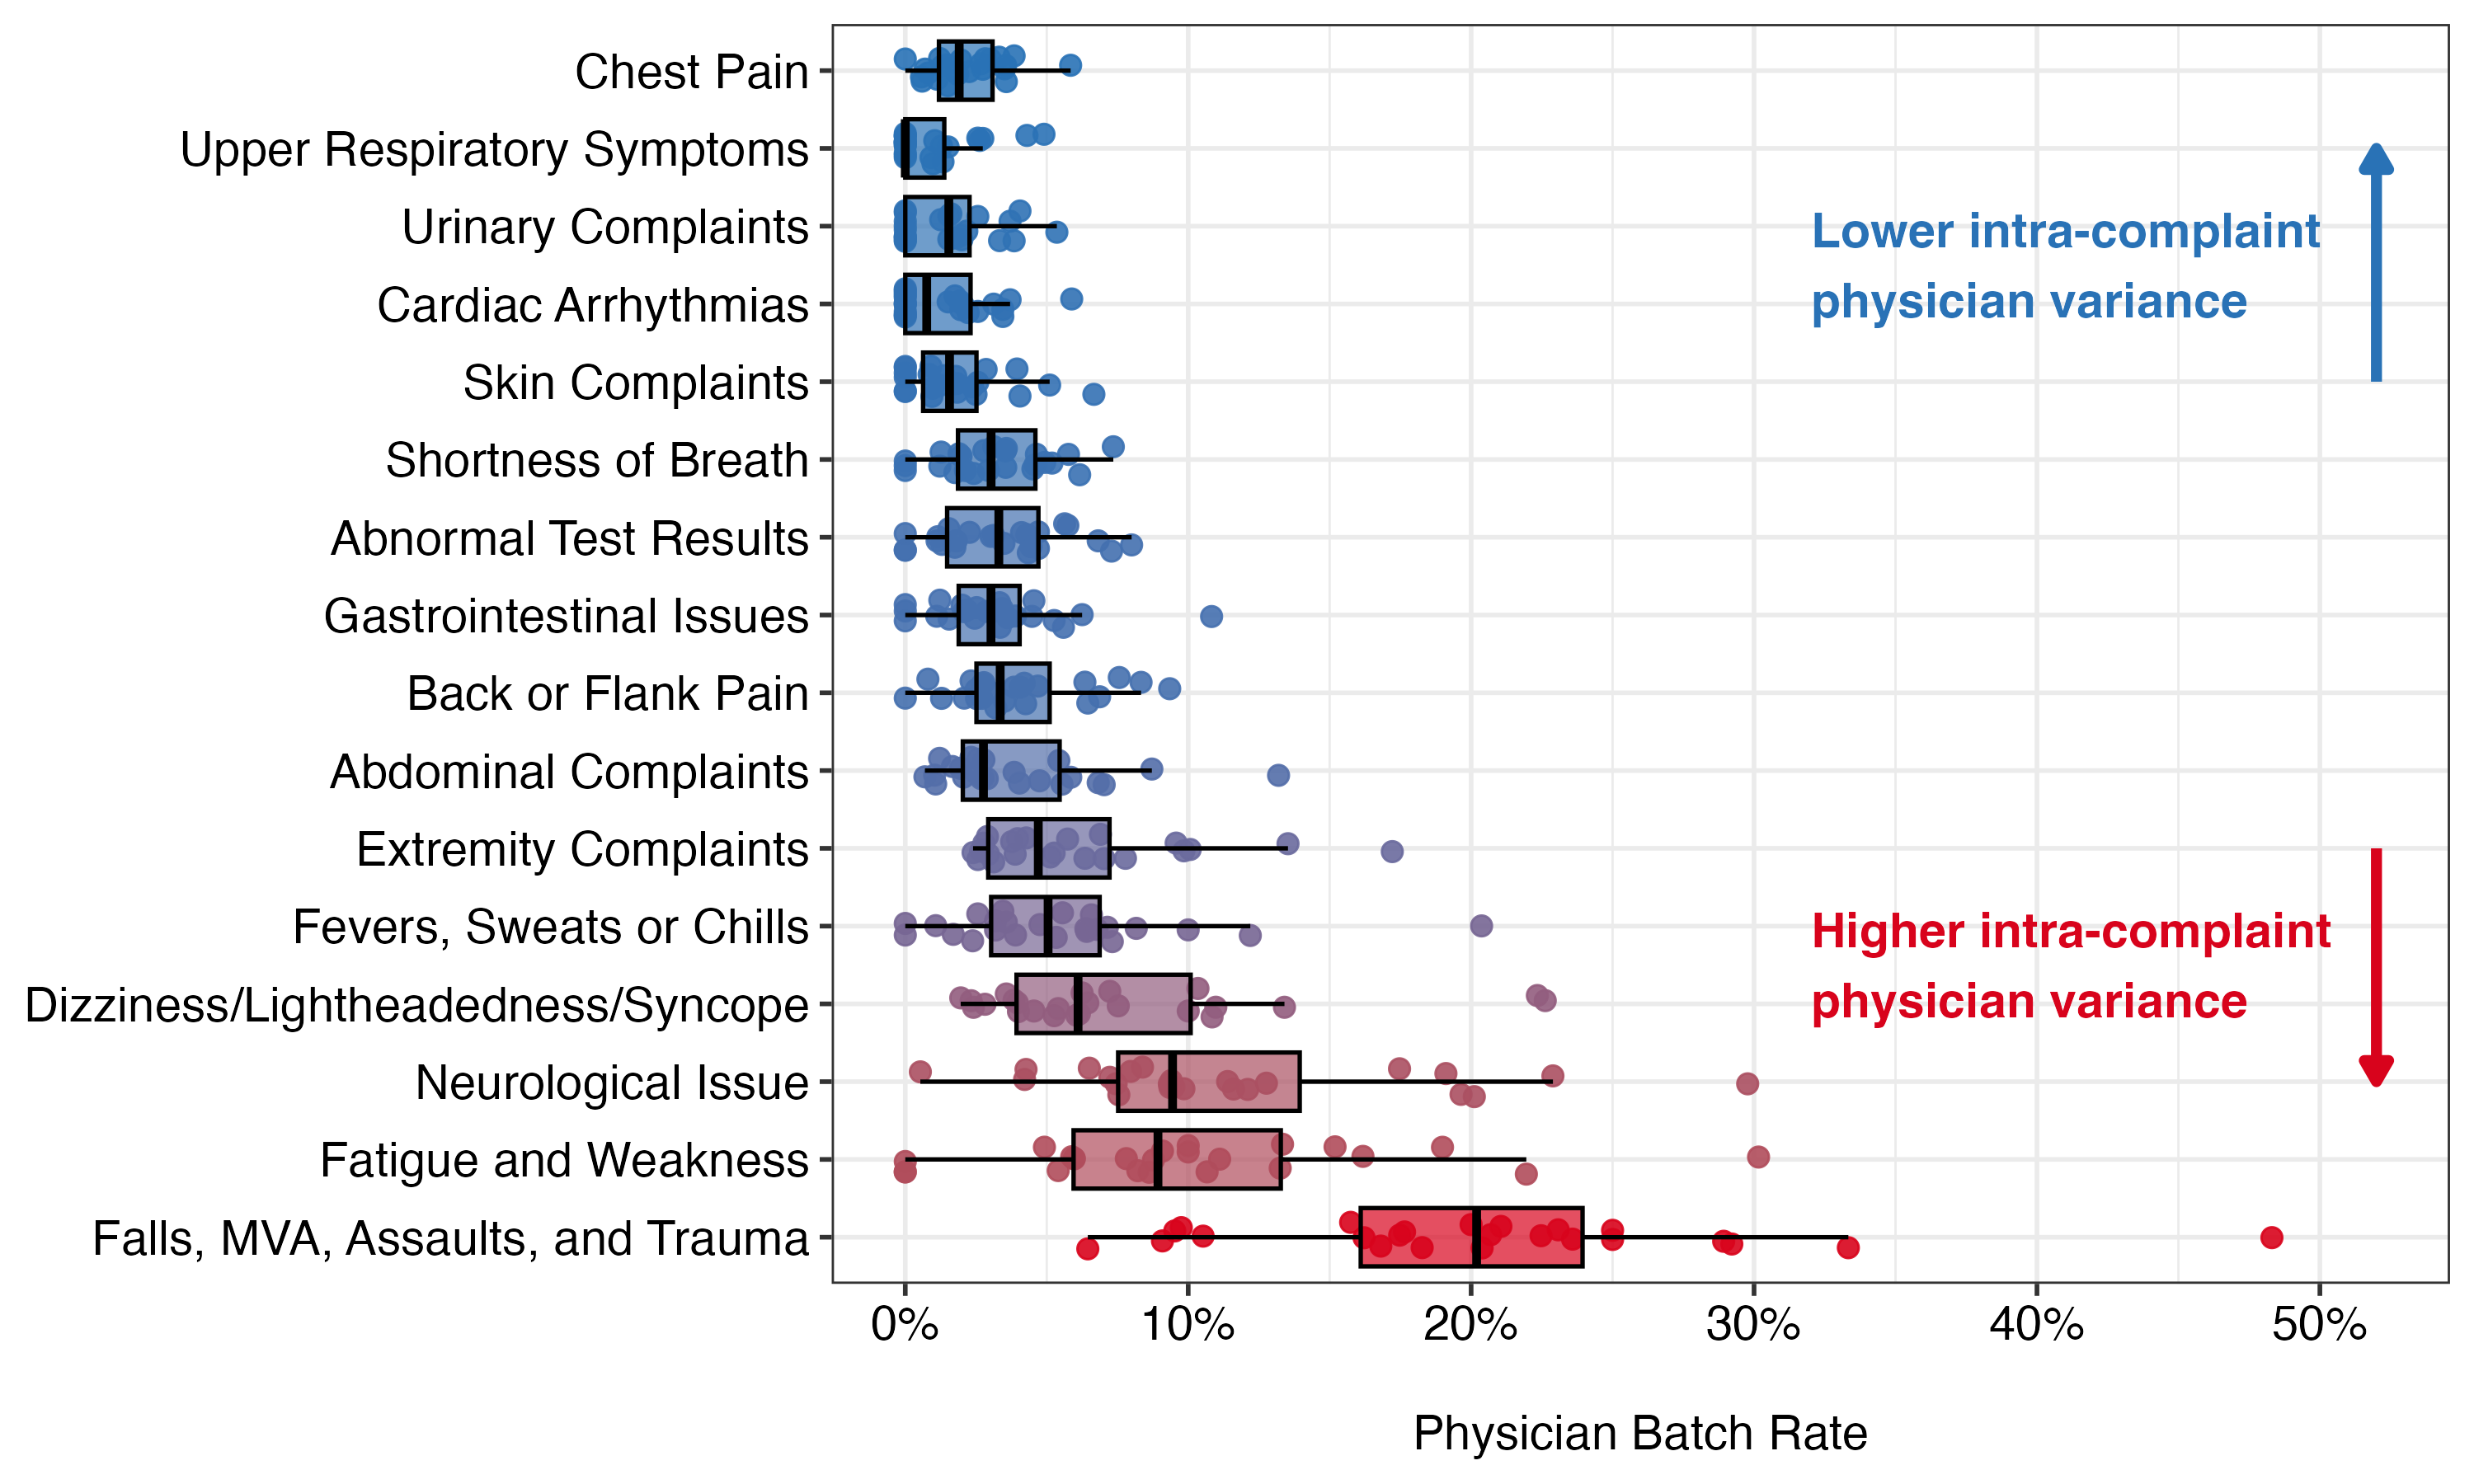
\includegraphics[width=\textwidth]{../outputs/figures/fig1_boxplot.png}
\label{fig:Variation}
\begin{tablenotes}
\item \footnotesize{\textit{Notes:} This figure highlights the marked differences among Mayo Clinic ED physicians in their propensity to batch order imaging tests. Batch rates are crude rates calculated by dividing the number of patient encounters where the physician batch ordered imaging tests for a complaint by the number of patient encounters they had with that complaint.}
\end{tablenotes}
\end{figure}

\begin{table}[h]
\centering
\caption{Descriptive Statistics of Emergency Department Encounters}
\label{tab:desc_stats}
\begin{threeparttable}
\begin{tabular}{p{9cm}cc}
\toprule
Variable & Mayo Clinic & MGH \\
 & (Median [IQR]) & (Median [IQR]) \\
Patients encounters$^a$ & n = 48,854 & n = 111,710 \\
\midrule
\textit{Panel A. Patient Severity} & & \\
Tachycardic & 19.2\% & 21.3\% \\
Tachypneic & 8.8\% & 5.4\% \\
Febrile & 2.2\% & 1.5\% \\
Hypotensive & 1.4\% & 1.0\% \\
Emergency Severity Index & 2.8 [2, 3] & 2.8 [2, 3] \\
\\
\textit{Panel B. Patient Demographics} & & \\
Male & 46.5\% & 51.3\% \\
Race: White & 88.4\% & 61.3\% \\
Race: Black & 4.2\% & 12.3\% \\
Race: Asian & 3.05\% & 4.89\% \\
Arrival age & 57.7 [43, 74] & 49.6 [32, 65] \\
\\
\textit{Panel C. Diagnostic Tests and Outcomes} & & \\
X-ray performed & 43.3\% & 40.1\% \\
Ultrasound performed & 11.3\% & 18.3\% \\
Non-contrast CT performed & 35.5\% & 30.5\% \\
Contrast CT performed & 17.7\% & 13.0\% \\
MRI performed$^{b}$ & --- & 6.3\% \\
Labs ordered & 73.7\% & 84.9\% \\
Time from arrival to triage (mins) & 8.0 [4, 10] & 12.2 [3, 13] \\
LOS (min) & 246 [152, 306] & 426 [241, 1006] \\
Time to disposition (min) & 246 [152, 306] & 426 [241, 1006] \\
Treatment Time (min) & 246 [152, 306] & 426 [241, 1006] \\
Patient discharged & 66.8\% & 65.1\% \\
Patient admitted & 18.7\% & 22.8\% \\
Patients revisited within 72 hours & 3.8\% & 3.1\% \\
Order to result$^{c}$: X-Ray (mins) & 67.2 [36, 79] & 63.4 [31.4, 111.7] \\
Order to result: Ultrasound (mins) & 165 [71, 150] & 119 [71, 213] \\
Order to result: Contrast CT (mins) & 142 [86, 153] & 167.3 [112.0, 260.6] \\
Order to result: Non-Contrast CT (mins) & 89.7 [50, 102] & 185.3 [116.0, 290.2] \\
Order to result: MRI (mins) & --- & 374.7 [229.5, 683.7] \\
\bottomrule
\end{tabular}
\begin{tablenotes}
\item \footnotesize \textit{Notes:} This table reports summary statistics for emergency department visits during the study period. Values are presented as mean (IQR) when available. Vital signs were categorized as follows: tachycardia (pulse more significant than $100$), tachypnea (respiratory rate greater than $20$), fever (temperature greater than $38^\circ C$), and hypotension (systolic blood pressure less than $90$).
\item \footnotesize $^a$The number of patient encounters is calculated as the number of unique patient visits during the study period.
\item \footnotesize $^b$MRI data is only available for MGH.
\item \footnotesize $^c$Order to result times are calculated as the difference between the time the test was ordered and the time the result was available in the electronic health record. This does not account for the time it takes for the radiologist to review the results.
\end{tablenotes}
\end{threeparttable}
\end{table}

Our empirical strategy closely follows the literature that relies on the
quasi-random assignment of agents to cases, often referred to as the
``judges design.'' \citep[\citet{dobbie2018effects}]{Dahl2014}. Studies
in this literature typically exploit variation in the sentencing
leniency of judges who work in the same court. Similarly, we exploit
batching variation across physicians who work in the same ED through a
measure we define as ``batch tendency.'' In its reduced form, under the
assumption of random or quasi-random assignment, this approach allows us
to identify the causal effect of being assigned to different types of
physicians (i.e., batcher or sequencer). Under additional assumptions,
an instrumental variable (as we will define it) allows us to estimate
the causal effect of the decision to batch on various measures of ED
performance.

Our instrumental variables approach provides us a local average
treatment effect (LATE) of batch ordering, which is the effect of batch
ordering on the subset of patients whose batching decision changes due
to the instrument. This is particularly important in the context of the
ED, where there are clear cases where batch ordering is necessary (e.g.,
when multiple tests are essential and almost every physician would
batch) and cases where it is not (e.g., when one or no tests are needed
and virtually no physician would batch). By estimating the effect for
the marginal patients whose tests may or may not be batched depending on
the provider, we generate more profound insights into the critical
implications of batch ordering as a result of physician discretion.

\subsection{Main Findings and
Contributions}\label{main-findings-and-contributions}

Despite the conventional wisdom that batching tests in the ED enables
physicians to gain efficiency, batch ordering imaging tests negatively
impacts operational metrics. In particular, our results show that the
marginal batched patient experiences a 130\% increase in total ED LOS
and an 123\% increase in time to disposition compared to patients who
have their tests ordered sequentially. Furthermore, when physicians
batch order imaging tests, they order 1.4 additional tests per patient
encounter compared to the sequential strategy. These effects remain
robust even after adjusting for patient characteristics, ED conditions,
and physician experience. Through mediation analysis, we find that the
increase in testing volume is a key driver of the increased LOS
associated with batch ordering. This effect of batching on LOS is
further mediated by the higher likelihood of admitting the patient,
which can increase LOS through boarding time.

Examining the drivers of batch ordering, we find that physicians are
more likely to batch order tests earlier in their shifts and for
patients with higher acuity levels and more complex chief complaints.
This batching tendency, however, varies systematically across physicians
and persists even after controlling for patient mix, ED conditions, and
observable physician characteristics. Finally, we find that ED crowding
significantly reduces the negative impact of batching behavior. For
example, during periods of major overcapacity, the effect of batching on
testing volume drops by nearly half compared to normal operations,
suggesting that resource constraints may induce batchers to be more
selective and exclude unnecessary tests from their batches.

Our results indicate that despite the perceived workflow advantages of
initiating multiple diagnostic processes simultaneously, batch ordering
leads to significantly longer processing times and increased resource
utilization without corresponding improvements in patient outcomes.
These findings have important implications, highlighting that ED
managers should consider strategies to reduce batching behavior to
improve diagnostic testing workflows. We shed light on such strategies
and provide actionable insights into ways ED managers can achieve this.

\section{Related Literature}\label{related-literature}

In EDs, physicians face a fundamental choice in how they sequence
diagnostic imaging tests: they can order multiple tests simultaneously
(``batch ordering'') or order them sequentially based on progressive
information gathering. Batch ordering occurs when a physician orders a
comprehensive set of diagnostic tests at the start of a patient
encounter, typically covering a broad range of potential diagnoses. This
contrasts with standard practice, where tests are ordered one at a time,
with each subsequent test decision informed by prior test results.

\subsection{Physician Decision-Making Under
Constraints:}\label{physician-decision-making-under-constraints}

ED physicians operate under significant time pressure and workload,
which substantially influence their decision-making processes. Workload
management and carefully balancing the tradeoffs between speed and
quality of care are of high importance for physicians making decisions
in a complex environment such as the ED
\citep[\citet{leppink2019mental}]{Saghafian2018} and lead to multiple
documented effects on physician performance. For instance, physicians
may resort to ordering additional diagnostic tests when faced with
limited patient interaction time, a practice requiring less immediate
critical thinking compared to direct clinical assessment
\citep[\citet{pines2009trends}]{batt2016early}.

Moreover, increased stress and frequent interruptions can disrupt
systematic decision-making and impair complex diagnostic reasoning
\citep[\citet{bendoly2011linking}]{chisholm2000emergency}. Frequent task
switching due to managing multiple simultaneous demands can exacerbate
cognitive strain and decision fatigue, prompting physicians to batch
diagnostic tests to defer intricate diagnostic decisions until
comprehensive results are available \citep[\citet{skaugset2016can},
\citet{jaeker2020value}]{kc2013does}. By ordering multiple tests
upfront, physicians can defer complex diagnostic reasoning until all
results are available, potentially reducing the cognitive strain of
repeated task-switching and decision-making under uncertainty. A
cognitive load theory of batching suggests that batching is more
prevalent during periods of high workload or complexity.

Significant variation in ED physician testing and admitting practices
has also been documented \citep[\citet{Coussens2024},
\citet{Smulowitz2021}]{hodgson2018are}. This variation also extends to
batch ordering, where physicians differ systematically in their
propensity to order multiple imaging tests simultaneously
\citep{jameson2024variation}. However, understanding the drivers and
operational impact of this variation remains a significant gap in the
literature. Our study aims to fill this gap by examining the factors
that drive batch ordering behavior and exploiting physician variation to
identify the causal effects of batch ordering on ED operations and
patient outcomes.

\subsection{Discretionary Behavior and Task Scheduling in Healthcare
Operations}\label{discretionary-behavior-and-task-scheduling-in-healthcare-operations}

Recent work has examined how operational factors influence physicians'
discretionary behavior in test ordering, revealing that decisions about
diagnostic intensity are shaped by multiple operational pressures
\citep{soltani2022does}. Studies have found that test utilization varies
with peer observation \citep{song2017closing}, workload \citep{Deo2019},
and the presence of justification requirements \citep{jaeker2020value}.
While additional tests can improve diagnostic accuracy, they also extend
ED LOS and potentially exacerbate congestion \citep{chan2018efficiency}.
This tension is particularly acute in imaging decisions, where test
sequencing can significantly impact patient flow and resource
utilization \citep{Cournane2016}.

The decision to batch order tests represents a specific form of
discretionary task ordering that has received limited attention in
healthcare operations. While prior work has examined discretionary task
ordering in other contexts \citep[\citet{Ibanez2020}]{Ibanez2018}, the
unique constraints of ED imaging--- including capacity limitations,
varying processing times across modalities, and the inability to run
different imaging types on a patient simultaneously--- make these
decisions particularly consequential. A growing literature examines how
workers exercise discretion over task ordering to improve system
performance \citep[\citet{Campbell2011}]{vanDonselaar2010ordering} but
also how such discretion can sometimes lead workers to ``choose the
wrong task operationally'' \citep{boudreau2003interface}.

The implications of batch ordering also connect to broader theoretical
work on task scheduling in resource-constrained environments. While
batching strategies often reduce setup times and improve throughput in
manufacturing settings \citep{Fowler2022}, applying these principles to
healthcare operations introduces unique complexities. While batching may
streamline the diagnostic process by initiating multiple diagnostic
processes simultaneously \citep{song2017closing}, recent evidence
suggests it may lead to increased testing volumes that could overwhelm
imaging departments and extend wait times
\citep[\citet{saghafian2015operations}]{Jessome2020}. The information
value of sequential testing--- where results from initial tests can
inform the necessity of subsequent ones--- creates a fundamental tension
between operational and diagnostic efficiency that has not been
well-studied. Our analysis provides novel evidence on this tradeoff,
showing how different test ordering strategies affect operational
metrics and clinical decision-making. Our study advances this literature
by providing causal evidence on how physicians' test sequencing
decisions affect ED performance. Furthermore, we identify specific
mechanisms through which batch ordering affects operational performance,
allowing us to distinguish between efficiency gains from parallel
processing and potential losses from increased diagnostic intensity.

\subsection{Hypothesis Development}\label{hypothesis-development}

Building on the literature reviewed above, we develop formal hypotheses
about how batch ordering affects ED operations. While prior work has
identified the mechanisms driving batching behavior and its potential
consequences, the net effects remain theoretically ambiguous. Our
theoretical framework centers on the fundamental tradeoff between the
perceived efficiency of parallel processing and the information value of
sequential testing.

\subsubsection{Information Value and Test
Volume}\label{information-value-and-test-volume}

The decision to batch or sequence tests fundamentally involves whether
to preserve the option value of information. Sequential testing allows
each test result to inform subsequent decisions, potentially eliminating
unnecessary tests. When physicians batch tests upfront, they commit to a
diagnostic pathway before information unfolds, forfeiting this option
value.

Physicians under high workload face cognitive strain from task switching
and may batch tests to defer complex diagnostic reasoning
\citep[\citet{skaugset2016can}]{kc2013does}. However, this cognitive
convenience comes at a cost. Without the filtering mechanism of
sequential information revelation, physicians must rely solely on their
initial assessment. \citep{lam2020why} identify this as a key driver of
overtesting---when facing diagnostic uncertainty, physicians order
comprehensive test batteries rather than allowing initial results to
guide subsequent testing. Given the documented variation in physician
testing intensity \citep{hodgson2018are}, with some physicians ordering
twice as many tests as their peers, batching likely amplifies these
tendencies by removing the natural stopping points that sequential
results provide. Therefore:

\begin{quote}
\small
\textit{\textbf{Hypothesis 1.} Batch ordering will increase the total number of imaging tests performed compared to standard practice due to the loss of information value from initial test results.}
\end{quote}

\subsubsection{Processing Time and Operational
Flow}\label{processing-time-and-operational-flow}

While batching strategies reduce setup times in manufacturing
\citep{Fowler2022}, the ED imaging context presents unique operational
constraints as noted in our review. Different imaging modalities require
separate equipment and cannot be performed simultaneously
\citep{Jessome2020}. This creates a fundamental bottleneck where batched
orders must still be executed sequentially, but now with a larger
committed workload that cannot be adjusted based on emerging
information.

Moreover, the cognitive load literature suggests that processing
multiple test results simultaneously increases decision complexity
\citep{kc2013does}. When physicians receive multiple results at once
rather than sequentially, they must integrate more information
simultaneously, potentially lengthening the diagnostic reasoning
process. This ``information overload'' effect, combined with the
additional tests ordered as predicted in H1, suggests that batching may
paradoxically increase rather than decrease processing times:

\begin{quote}
\small
\textit{\textbf{Hypothesis 2.} Batch ordering will increase patient length of stay and time to disposition compared to standard practice, as the operational constraints of imaging and increased test volume outweigh any potential benefits of parallel processing.}
\end{quote}

\subsubsection{Clinical Decision-Making and
Disposition}\label{clinical-decision-making-and-disposition}

The medical literature recognizes ``diagnostic momentum''---where
abnormal findings, even if clinically insignificant, drive further
workup and more conservative clinical decisions
\citep[\citet{featherston2020decision}]{coen2022clinical}. When
physicians batch order and receive multiple results simultaneously, they
encounter more opportunities for incidental findings that may influence
disposition decisions
\citep[\citet{berlin2011incidentaloma}]{lumbreras2010incidental}. As our
review noted, physicians facing uncertainty and potential legal
consequences may opt for more conservative disposition decisions
\citep[\citet{lam2020why}]{rao2012overuse}. The simultaneous arrival of
multiple test results, particularly with incidental findings, may
trigger defensive medicine behaviors:

\begin{quote}
\small
\textit{\textbf{Hypothesis 3.} Batch ordering will increase hospital admission rates through increased diagnostic intensity and the influence of incidental findings on clinical decision-making.}
\end{quote}

\subsubsection{Contextual Moderators}\label{contextual-moderators}

The literature on physician behavior under capacity constraints
consistently shows that resource scarcity forces more selective
decision-making \citep[\citet{kc2009impact}]{kuntz2014stress}. When EDs
face severe overcrowding, the operational pressures documented in our
review intensify. Under these conditions, physicians may reserve
batching for cases where it is clinically essential rather than
convenient:

\begin{quote}
\small
\textit{\textbf{Hypothesis 4.} The effects of batch ordering on LOS and test volume will be attenuated under conditions of major ED overcapacity, as physicians become more selective in their batching decisions.}
\end{quote}

These hypotheses provide testable predictions that we examine using our
quasi-experimental design. By leveraging variation in physician batching
tendency under random patient assignment, we can identify whether these
theoretical mechanisms manifest in actual ED operations.

\section{Setting, Data, and Models}\label{sec:3}

\subsection{Empirical Setting}\label{sec:4.1}

Our study uses data from two large U.S. emergency departments (EDs): the
Mayo Clinic of Arizona and Massachusetts General Hospital (MGH). The MGH
dataset, which includes 129,489 patient encounters from November 10,
2021, through December 10, 2022, provides a robust sample for validating
the generalizability of our findings. However, our primary analysis
focuses on the Mayo Clinic data due to its unique feature of random
patient-physician assignment, which allows for stronger causal
inference. More specifically, the Mayo Clinic ED employs a sophisticated
computerized rotational patient assignment algorithm that addresses many
of the empirical challenges previously identified
\citep{Traub2016, traub2016emergency, Traub2018}. The system
automatically assigns patients to physicians 60 seconds after
registration through the electronic health record system, following a
strict rotational protocol. At shift start, each physician receives four
consecutive patients to establish an initial patient load, after which
they enter rotation with other on-duty physicians. Critically, these
assignments are based solely on arrival time---the algorithm does not
consider patient demographics, chief complaint, Emergency Severity Index
score, physician workload, or the acuity of recently assigned patients.
To maintain system integrity, physicians receive no new patients during
their final 120 minutes and are capped at 18 patients per shift. The
rotation order follows a predetermined schedule that varies across
shifts to ensure fairness over time.

This rotational mechanism achieves the quasi-randomization necessary for
causal inference. Unlike settings where patient-physician matching may
be influenced by triage decisions, physician preferences, or informal
routing practices, the Mayo Clinic's algorithmic assignment removes
discretion from the matching process. We establish that, conditional on
arrival time, patient-physician matching is effectively random---a
critical requirement for our identification strategy that distinguishes
our study from observational analyses where endogenous matching could
confound the effects of physician discretion.

The data contain information on the timing of test orders, test results,
and patient disposition, among various other important triage metrics
and demographic features. We focus on imaging tests (x-rays, contrast CT
scans, non-contrast CT scans, and ultrasound) because, unlike laboratory
tests, these tests cannot be run simultaneously on a given patient due
to the different equipment and settings required. Therefore, the
operational implications of batch ordering imaging tests are more
pronounced. We exclude MRI from our Mayo analysis due to an
institutional policy requiring either inpatient admission for urgent
MRIs or outpatient ordering for non-urgent cases, resulting in
negligible ED MRI usage. MGH does not have this policy, so we included
MRI in their generalizability analysis.

\subsection{Data}\label{data}

Our primary data comes from the Mayo Clinic of Arizona ED, a tertiary
care hospital without obstetrical services, an inpatient pediatrics
unit, or a trauma designation. During the study period (October 6, 2018,
through December 31, 2019) the ED recorded 48,854 visits during the
study period, managed across 26 treatment rooms and up to 9 hallway
spaces. The department is exclusively staffed by board-eligible or
board-certified emergency physicians (EPs), a rare but ideal setting for
our study. Many EDs are staffed by a mix of EPs and non-EPs (e.g., Nurse
Practitioners and Physician Assistants), both responsible for ordering
tests, which may introduce confounding factors. The Mayo Clinic ED is
unique in that only EPs can order tests, eliminating the potential for
confounding by provider type. Furthermore, as mentioned earlier, the ED
makes uses of a randomized patient to EP assignment, eliminating some
other potential sources of confounding.

We conducted a retrospective review of the comprehensive ED operations
data, coinciding with the initiation of a new electronic medical record.
The data includes detailed patient demographics, chief complaints, vital
signs, emergency severity index (ESI), LOS, timestamps, and resource
utilization metrics. This period was chosen to provide a robust data set
while excluding the influence of the coronavirus pandemic. The data is
summarized in Table \ref{tab:desc_stats}. Hourly patient arrival rates
to the ED are shown in Appendix Figure A1. LOS is measured from the time
of arrival to departure from the ED. During periods when inpatient beds
are filled to capacity (i.e., when patients requiring inpatient
admission must ``board'' in the ED due to lack of inpatient beds), the
Mayo Clinic converts ED beds into temporary inpatient beds, making the
endpoint for LOS for ED boarders when they are moved from their ED bed
to their assigned ``inpatient'' boarding bed within the ED
\footnote{The Mayo Clinic hospital operations team views ED crowding and boarding as a hospital-wide problem and not an ``ED problem," and they have elected to convert multiple sites around the hospital including pre-operative areas into boarding areas during hospital overcapacity instead of the ED, assigning ED to be the location of boarders as a true last resort.}.

To improve power in our analyses, we drop encounters with rare ``reasons
for visit'' (RVF) (defined as those with less than \(1000\) total
encounters) as well as complaints where either a batch order occurs less
than \(5\%\) of the time across all patients or no imaging is ordered.
Since batch orders are rare for these cases, our physician batch
tendency instrument could suffer from a weak instrument problem if we
included them. Examples of complaints dropped include skin and urinary
complaints, as well as other complaints where multiple imaging
modalities are unlikely to occur. Excluding these conditions does not
introduce selection bias because of the random assignment. Finally, to
estimate a precise measure of physician-level batch tendency, we
restrict our sample to the encounters only involving full-time
physicians. Our final sample includes 11,404 encounters consisting of
chief complaints from the following categories: Neurological Issue,
Abdominal Complaints, Fevers, Sweats or Chills, Falls, Motor Vehicle
Crashes, Assaults, and Trauma, Dizziness/Lightheadedness/Syncope,
Extremity Complaints, and Fatigue and Weakness.

\subsubsection{Treatment Variable}\label{treatment-variable}

Our treatment variable, \(Batched_{i,t}\), is an indicator taking the
value of \(1\) if patient \(i\) has their tests batch ordered during
their ED encounter, which took place on date \(t\), and \(0\) otherwise.
Batching occurs when a physician simultaneously orders a comprehensive
set of diagnostic tests, typically covering a broad range of potential
diagnoses. This contrasts with standard care, where a single test is
ordered and subsequent tests are ordered in sequence on an as-needed
basis.

We define ``batching'' in line with standard emergency medicine
practices and focus on batches that include two or more different
imaging modalities where the time between orders is within 5 minutes,
occurring as the first imaging tests ordered for the patient encounter
\citep[\citet{jameson2024variation}]{su2025crisis}. We focus on batches
that concern the first imaging tests ordered during the patient
encounter because this represents the moment of maximum diagnostic
uncertainty when physicians must decide their testing strategy before
clinical information unfolds. Physicians cannot know ex-ante which
patients will ultimately require multiple tests, making early batching a
discretionary choice based on practice style rather than clinical
necessity. Each imaging modality, such as X-ray, contrast CT scan,
non-contrast CT, and ultrasound, is considered a separate and distinct
test for our study. In particular, we focus on batching instances where
the physician orders different imaging tests because such tests cannot
be done in a single scanning session (due to differences in equipment
and setting). Encounters where a single test precedes subsequent batched
tests (1.91\% of multi-test cases) are classified as sequential in our
primary analysis, as the physician has initiated sequential information
gathering before placing additional orders. Sensitivity analyses
conducted around this time window, batch size threshold, and the timing
of the batch show that our results are robust to variations in these
values.

\subsubsection{Dependent Variables}\label{dependent-variables}

The primary outcomes of interest are the ED's efficiency and
effectiveness measures. The first is patient length of stay, which we
measure in two ways. First, we measure the time from patient arrival
until the attending physician completes care and determines disposition,
capturing the duration until a decision is made to admit, discharge, or
transfer the patient \citep{Feizi2023}. This metric excludes delays
related to inpatient bed availability, providing a more transparent
measure of ED operational efficiency. Second, we measure a patient's
total time in the ED from arrival until physical departure
\citep{Lim2024}. This total time for admitted patients includes the
duration until transfer to an ``inpatient'' bed, whether in the main
hospital or designated ED areas converted for inpatient use,
encompassing boarding time and discharge processing \citep{Feizi2023}.
Given the documented right-skewed nature of ED time metrics
\citep{Song2015}, we log-transform both time measurements to achieve
approximately normal distributions
\citep[\citet{Saghafian2024}]{Brown2005}, meeting the assumptions
required for our regression analyses.

Beyond time-based metrics, we examine resource utilization through the
number of distinct imaging tests ordered during each ED encounter. This
count variable helps us understand how batch ordering practices
influence the diagnostic workload. To assess the quality of care, we
track whether patients return to the ED within 72 hours of their initial
visit and require hospital admission \citep{Lerman1987}. This binary
indicator is a crucial quality metric, as returns within this timeframe
may signal potential issues with initial treatment decisions, premature
discharges, or missed diagnoses. These measures are widely used and
validated in the emergency medicine literature and are also of
significant concern to our partner EDs. Furthermore, they allow us to
evaluate ED performance across three critical dimensions: operational
efficiency through time-based measurements, resource utilization via
imaging orders, and care quality through return visit patterns. By
examining these outcomes together, we can assess how batching behaviors
and related process changes affect the efficiency and effectiveness of
care delivery.

\subsection{Identification Strategy}\label{sec:identification}

Our empirical strategy closely follows the literature that relies on the
quasi-random assignment of agents to cases, often referred to as the
``judges design.'' Papers in this literature typically exploit variation
in the sentencing leniency of judges who work in the same court.
Similarly, we explore batching variation across physicians who work in
the same ED via a measure that we term ``batch tendency.'' We use each
physician's residualized leave-out average batch rate to measure
physician batch tendency. We use this residualized measure of physician
batch tendency because if certain physicians are more likely to work
afternoon or weekend shifts (Figure A1 shows to be the busiest shifts),
the simple leave-out mean will be biased. A residualized measure of
physician batch tendency accounts for this potential selection. This
measure is derived from two steps following a similar approach used in
other applications (e.g., \citet{doyle2015measuring},
\citet{dobbie2018effects}, and \citet{eichmeyer2022pathways}). First, we
obtain residuals from a regression model, which includes all ED
encounters in our sample period:

\begin{equation}
Batched_{i,t} = \alpha_0 + \alpha_{ym} + \alpha_{dt} + \mathbf{\beta X_{i,t}} + \varepsilon_{i,t},
\end{equation}

where \(Batched_{i,t}\) is a dummy variable equal to one if patient
\(i\) had their imaging tests batch ordered on an encounter on date
\(t\). Fixed effects include year-month fixed effects, \(\alpha_{ym}\),
to control for time and seasonal variation in batching,
hospital-specific policies (e.g., initiatives to eliminate excess
testing during a flu season), or seasonality in ED visits. We also
control for ``shift-level'' variations that include both physician
scheduling and patient arrival with day of week-time of day fixed
effects,
\(\alpha_{dt}\)\footnote{Day of week takes on seven values: Sunday, Monday, etc., and time of day are six mutually exclusive four-hour bins: 8 am–12 pm, 12 pm–4 pm, etc.}.
A vector of patient characteristics, \(\mathbf{X_{i,t}}\), including
chief complaint by ESI, vital signs, age, race, and sex, was included to
increase precision. As stated in \ref{sec:4.1}, these controls are more
than required for our quasi-random assignment assumption. Under the
assumption that we have captured the observables under which
quasi-random assignment occurs in the ED, the unexplained variation---
the physician's contribution--- resides in the error term,
\(\varepsilon_{i,t}\).

In step two, the tendency measure for patient \(i\) seen by physician
\(j\) is computed as the average residual across all other patients seen
by the physician during the study period:

\begin{equation}
Batch Tendency_{i,j}^{phys} =
\frac{1}{N_{-i,j}} \sum_{i' \in \{\mathbb{J} \backslash i\}}\hat{\varepsilon}_{i'}
\end{equation}

where \(\hat{\varepsilon}_{i'} = \hat{Batch}_{i'} - Batch_{i'}\) is the
residual from Eq. (1); \(\mathbb{J}\) is the set of all ED encounters
treated by physician \(j\); and
\(N_{-i,j} = |\{\mathbb{J} \backslash i\}|\), the number of cases that
physician has seen that year, excluding patient \(i\). This leave-out
mean eliminates the mechanical bias that stems from patient \(i\)'s case
entering into the instrument. The measure is interpreted as the average
(leave-out) batch rate of patient \(i\)'s physician relative to other
physicians in that hospital-year-month, hospital-day of week-time of
day.

Figure \ref{fig:batch_tendency} provides empirical verification that,
while the decision to batch depends on patient characteristics, our
measure---batch tendency---is plausibly exogenous. The left panel uses a
linear probability model to test whether encounter, patient, ED, and
physician characteristics predict the batching decision, controlling for
shift-level fixed effects with standard errors clustered at the
physician level. As expected, patient characteristics strongly predict
batching decisions; for instance, patients with Falls/Assaults/Trauma
complaints are 16.2 percentage points more likely to be batched compared
to similar patients under similar ED capacity. The right panel assesses
whether these same characteristics predict assignment to physicians with
different batch tendencies. Importantly, we find that patient
characteristics do not significantly predict assignment to high versus
low batch-tendency physicians. The coefficients are near zero with
confidence intervals crossing zero for all patient characteristics,
confirming that, conditional on shift fixed effects (which account for
the mechanical rotation), the assignment of patients to physicians with
different batching tendencies is effectively random. This validates the
rotational assignment mechanism and establishes batch tendency as an
exogenous source of variation for identifying causal effects.

\begin{figure}[t]
\caption{Batch Tendency by Patient Characteristics}
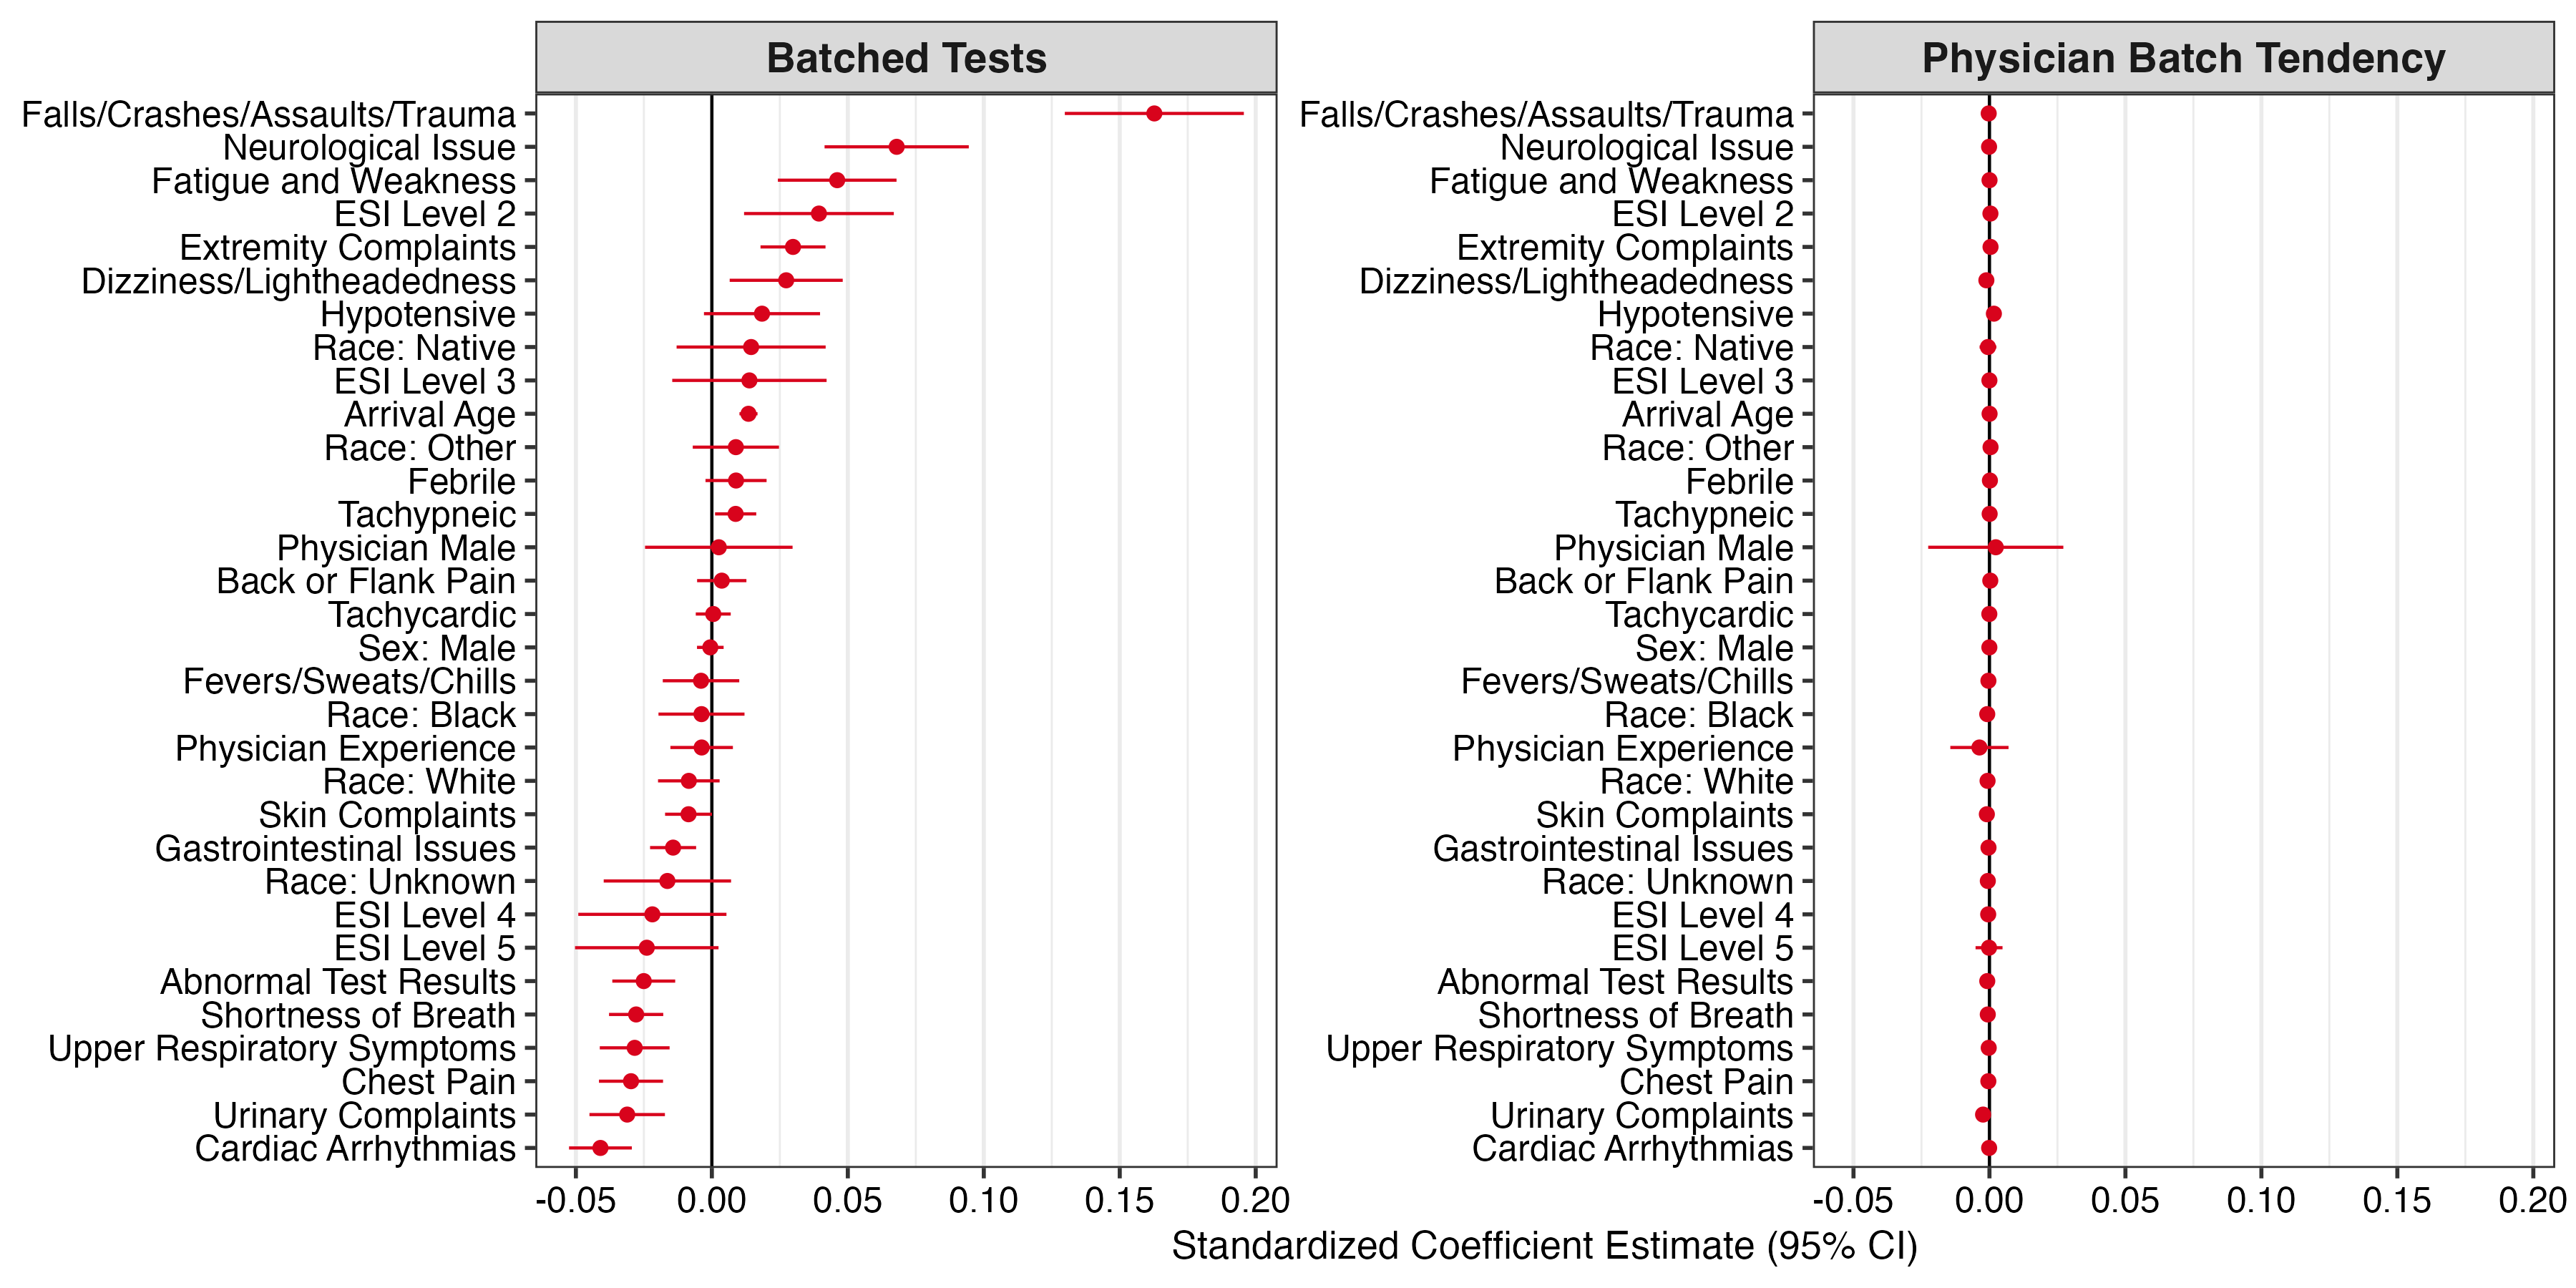
\includegraphics[width=\textwidth]{../outputs/figures/fig2_panel_batched_standardized.png}
\label{fig:batch_tendency}
\begin{tablenotes}
\item \footnotesize \textit{Notes:} This figure plots a test for quasi-random assignment of patients to physicians in the Mayo Clinic ED. Residualization fixed effects include hospital-year-month, hospital-day of week-time of day. Robust standard errors are clustered at the physician level.
\end{tablenotes}
\end{figure}

We further document that (a) there is significant variation in this
measure, and (b) the measure is highly predictive of the decision to
batch. Figure \ref{fig:tendency} shows the distribution of physician
batch tendency and the relationship between batch tendency and batching,
where the relationship is illustrated via local linear regression of
batching against physician tendency. As can be seen, the probability of
batching is monotonically and approximately linearly, increasing in our
tendency measure (see Table \ref{tab:first_stage} for more formal
results).

\begin{figure}[t]
\begin{center}
\caption{Distribution and First Stage of Instrument}
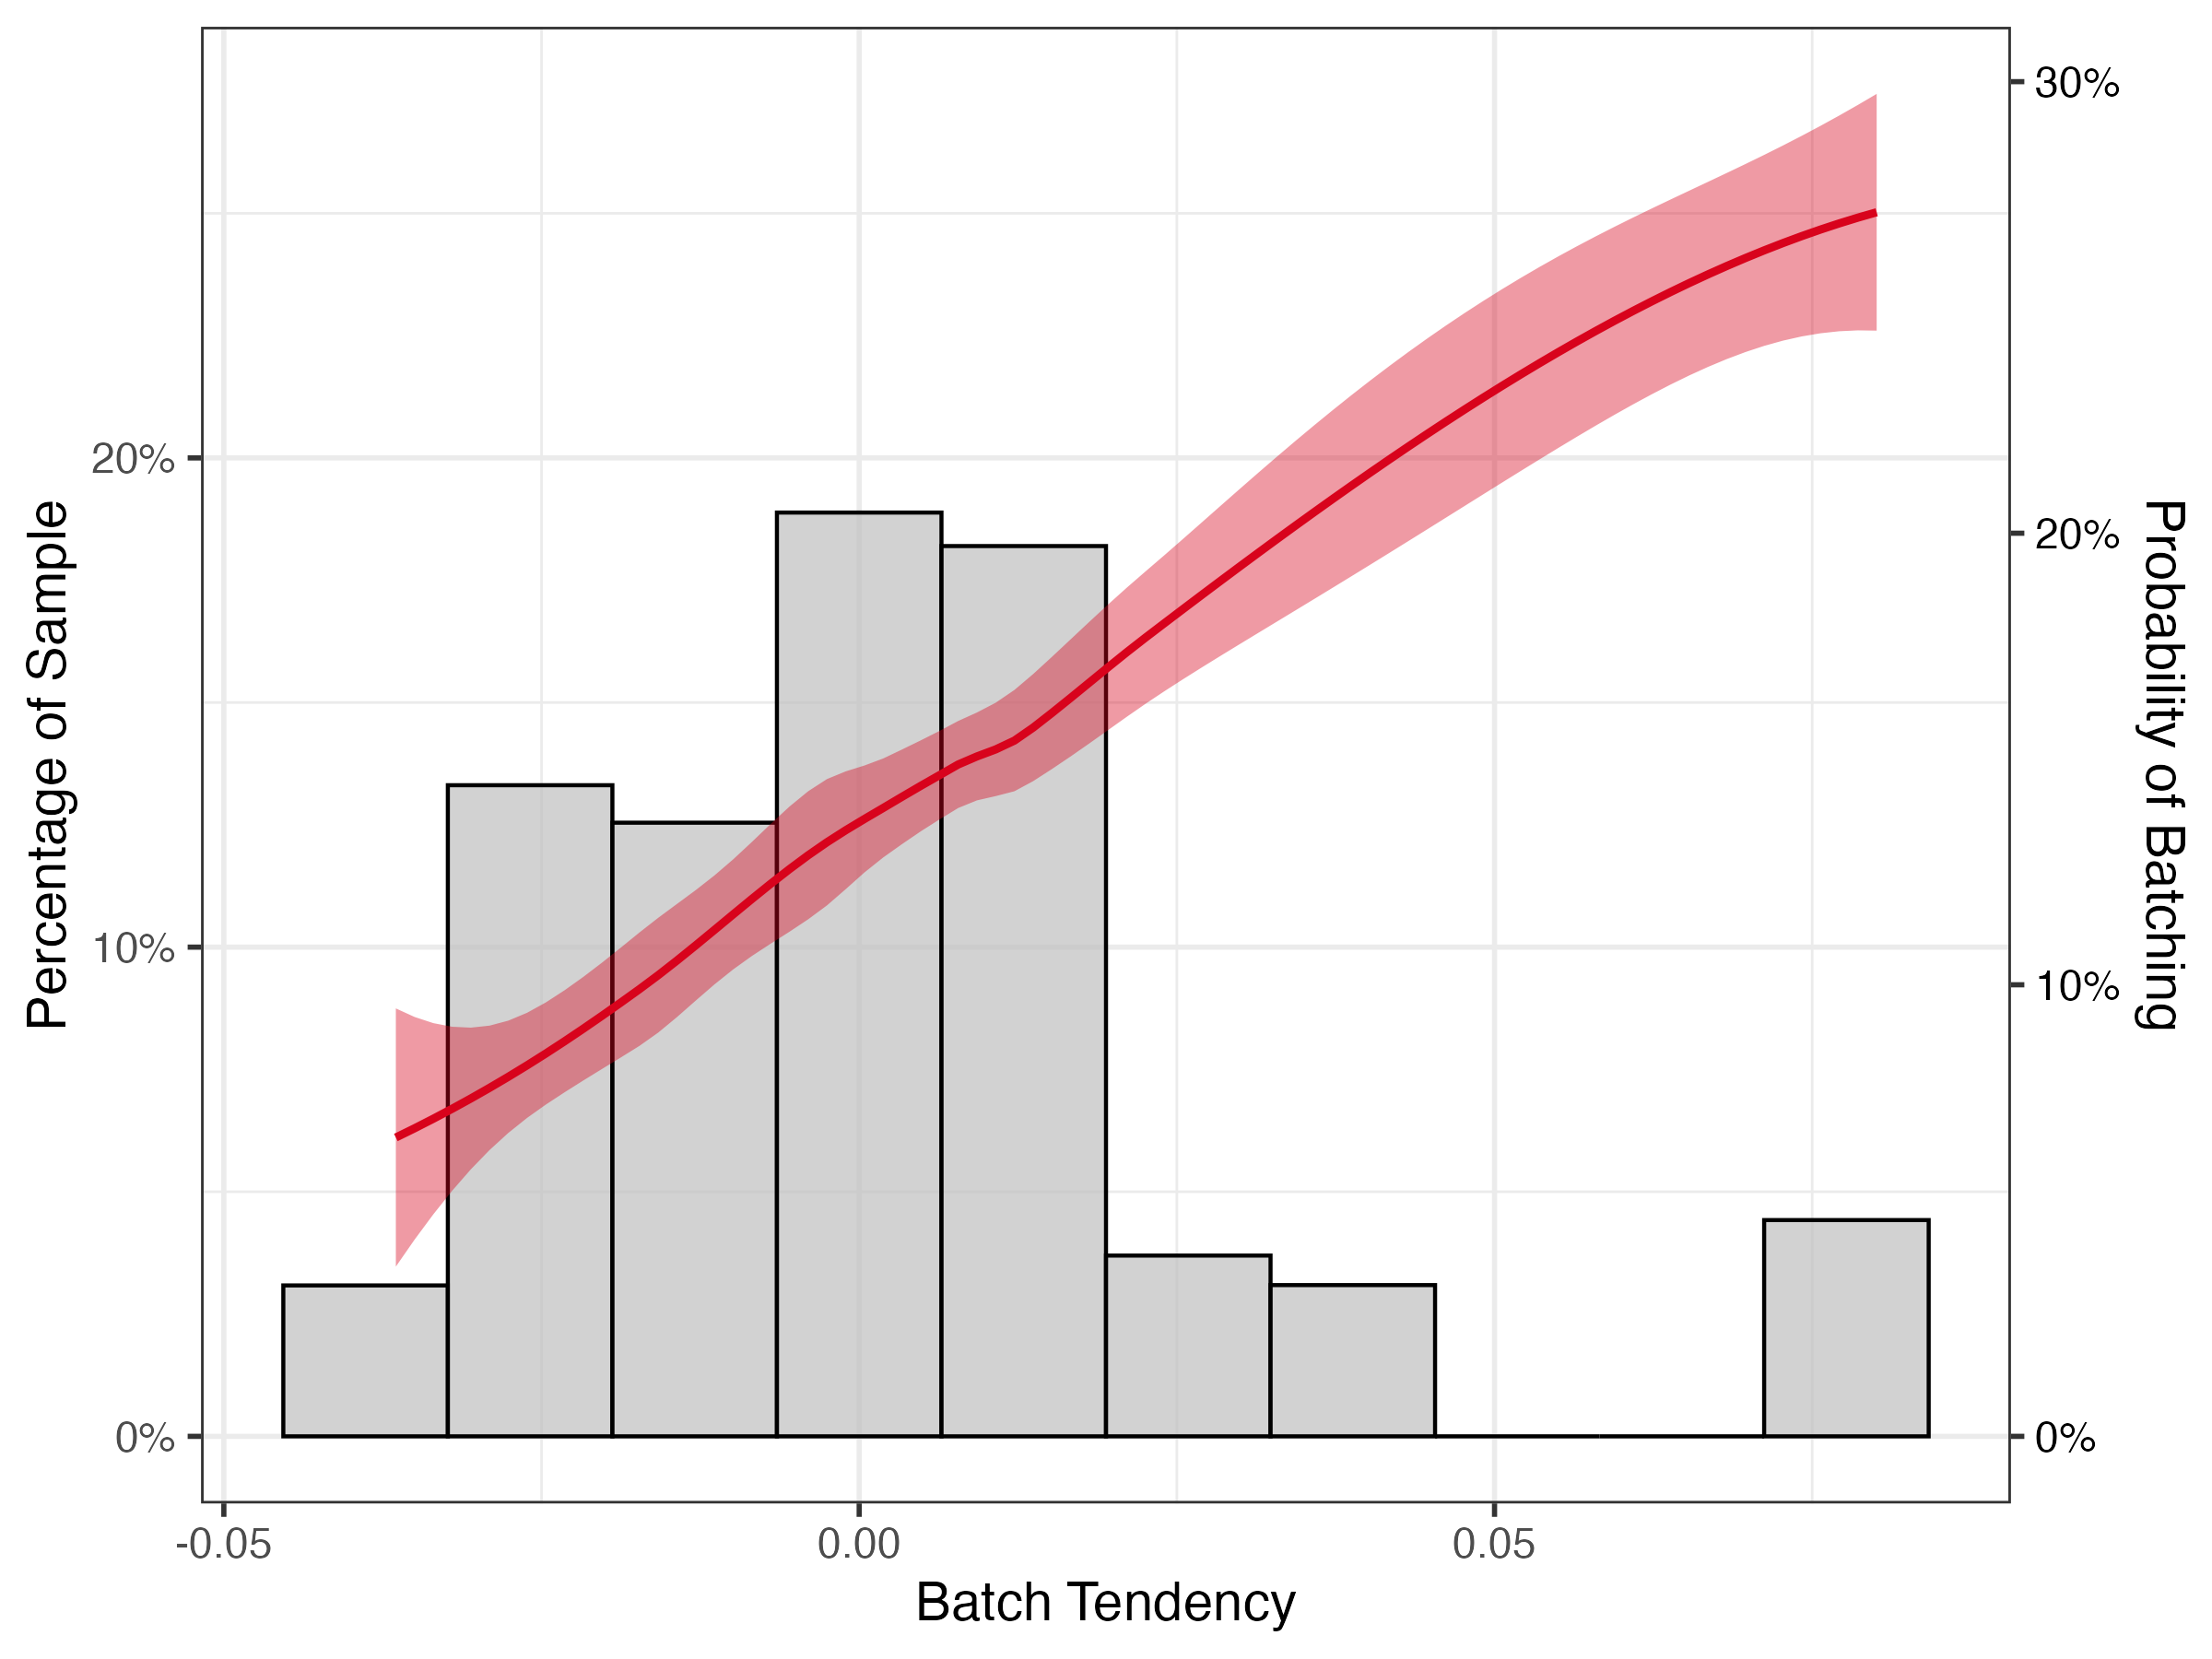
\includegraphics[width=0.65\textwidth]{../outputs/figures/Fig3_firststage.png}
\label{fig:tendency}
\end{center}
\begin{tablenotes}
\item \footnotesize \textit{Notes:} This figure plots the histogram of physician batch tendency along the x-axis and the left y-axis for all patient encounters. A local-linear regression of the fitted probability of batching on batch tendency after residualizing (see text for baseline fixed effects and controls in residualization) is overlaid and displayed on the right y-axis. Ninety-five percent confidence bands are also shown.
\end{tablenotes}
\end{figure}

Together, we observe that batch tendency likely satisfies the conditions
required for a valid IV. In the next section, we formalize our IV
analysis questions and more formally establish the validity of our IV.

\subsubsection{IV Analysis}\label{iv-analysis}

To estimate the reduced-form effects of being treated by a
batch-preferring physician (batcher), we estimate the following
equation:

\begin{equation}
Y_i = \mu_0 + \mu_1 \, BatchTendency_{i,j}^{phys} + \mathbf{\gamma X_i} + \nu_i
\end{equation}

To study the effects of test batching on outcomes, \(Y_i\), we estimate
the following Two-Stage Least Squares (2SLS) equations:

\begin{equation}
\left\{
\begin{aligned}
\text{First Stage:} \quad & Batched_i = \delta_0 + \delta_1 \, BatchTendency_{i,j}^{phys} + \mathbf{\delta_2 X_i} + \nu_i \\
\text{Second Stage:} \quad & Y_i = \beta_0 + \beta_1 \hat{Batched_i} + \mathbf{\theta X_i} + \varepsilon_i
\end{aligned}
\right.
\end{equation}

In all cases, \(Y_i\) represents our primary outcomes of interest, and
\(\mathbf{X_i}\) includes the same covariates as in Eq. 1 and additional
controls for physician experience, physician sex, and ED capacity level
(ED capacity guidelines for Mayo Clinic are in Appendix Table A1. The
variable \(Batched_i\) may suffer from potential endogeneity concerns;
for example, injury severity may be unobserved and correlated with the
need to run multiple tests, length of stay, and return with admission
likelihood. Hence, we instrument \(Batched_i\) with the assigned
physician \(j\)'s underlying tendency to batch,
\(BatchTendency_{i,j}^{phys}\). We cluster robust standard errors at the
physician level to account for the assignment process of patients to
physicians.

Table \ref{tab:first_stage} presents formal first-stage results from Eq.
(4). Column 1 of Table 2 presents the mean crude batch rate. Column 2
begins by reporting results only with year-month and
day-of-week-time-of-day fixed effects. Column 3 adds our baseline
patient and hospital condition controls. Consistent with Figure
\ref{fig:tendency}, our residualized physician instrument is highly
predictive of whether a patient will have their imaging tests batch
ordered. Including controls in column 3 does not change the magnitude of
the estimated first-stage effect, consistent with the quasi-randomness
of patients to physicians with different batching tendencies.

Furthermore, the batch tendency measure reasonably predicts the batching
decision and the IV is not weak (F values are 520.4 and 227.6 for
columns 2 and 3, respectively). For example, with all controls (column
3), our results show that a patient assigned to a physician that is at
the 90th percentile of batch tendency (0.023) relative to a physician at
the 10th percentile (-0.024) is 8.7 percentage points more likely to
have their tests batched. The coefficient is greater than one because
all emergency visits are used to construct the tendency instrument. The
first stage is calculated using only the baseline sample, excluding the
rare and rarely batched complaints.

\begin{table}[ht]
\centering
\caption{First-Stage Results: Batch Tendency and Batching}
\label{tab:first_stage}
\begin{threeparttable}
\begin{tabular}{p{8cm}ccc}
\toprule
 & Sample Mean & \multicolumn{2}{c}{Batched} \\
\cmidrule(lr){3-4}
 & (1) & (2) & (3) \\
\midrule
Batch Tendency & 0.136 & $1.855^{***}$ & $1.854^{***}$ \\
 & (0.342) & (0.081) & (0.123) \\
\midrule
\textit{Controls} \\
Shift-level Fixed Effects & --- & Yes & Yes \\
Baseline Controls & --- & No & Yes \\
\midrule
Adj. $R^2$ & --- & 0.023 & 0.064 \\
F-stat & --- & 520.4 & 227.6 \\
Observations & 11,404 & 11,404 & 11,404 \\
\bottomrule
\end{tabular}
\begin{tablenotes}
\footnotesize
\item \textit{Notes:} This table reports first-stage results for the regression of batch tendency on the likelihood of batching. Column 1 reports the sample mean and standard deviation of the dependent variable. Column 2 includes fixed effects for year-month and day of week-time of day. Column 3 adds baseline controls, including patient characteristics (age, vital signs like tachycardia, tachypnea, febrile, hypotensive status), hospital characteristics (capacity level), and physician characteristics (physician sex and physician experience). Robust standard errors are clustered at the physician level.
\item $^{***} p < 0.01$.
\end{tablenotes}
\end{threeparttable}
\end{table}

\subsubsection{Identifying
Assumptions}\label{sec:identifying_assumptions}

The reduced-form approach delivers an unbiased estimate of the causal
effect of being treated by a physician with a higher tendency to batch
since patient assignment to ED physicians is random and conditional on
seasonality and shift (``conditional independence''). The
residualization in Eq. (1) allows for further statistical precision in
measuring physician tendency to batch.

Our instrumental variable approach, which aims to recover the causal
effect of having diagnostic tests batch ordered, relies on three
additional assumptions: relevance, exclusion, and monotonicity. We
reported a strong first stage (i.e., relevance) at the end of the
previous section. The exclusion restriction requires the instrument to
influence the outcome of interest only through its effect on test
batching. This is our strongest assumption and is, at its core,
untestable. Nevertheless, we take this assumption seriously and perform
a placebo check in Appendix D1 and various robustness checks in Section
\ref{sec:robustness}.

However, several features of the ED setting suggest that such violations
may likely only have a small impact and may be less concerning than in
other healthcare settings. First, unlike in primary care settings, where
the patient and primary care provider have many repeated encounters, the
scope of what the emergency physician can do to impact medium-term
outcomes is limited and well-observed by the researcher. Second, any
exclusion restriction violation must directly affect the specific
outcome of interest. The channel by which ED physicians can influence
the outcomes of interest is likely through testing and diagnosis. To the
extent that the exclusion restriction is violated, our reduced form
estimates can be interpreted as the causal impact of being assigned to a
more or less likely to batch physician. Table \ref{tab:red_form} shows
these reduced form results.

Finally, the monotonicity assumption is necessary for interpreting the
coefficient estimates obtained from the IV approach as LATEs if there
are heterogeneous treatment effects. It requires that any patient whom a
low batch tendency physician batches would also be batched by a high
batch tendency physician. The literature leveraging the judges design
typically performs two informal tests for its implications. The first
one provides that the first stage should be weakly positive for all
subsamples (\citet{dobbie2018effects}). The second implication asserts
that the instrument constructed by leaving out a particular subsample
has predictive power over that same left-out subsample
(\citet{bhuller2020incarceration}). Appendix Figure D1 presents both of
these tests for various subsamples of interest. In the left panel, our
residualized measure of batch tendency is consistently positive and
sizable in all subsamples, which aligns with the monotonicity
assumption. In the right panel, we also find that our additional
first-stage results are consistently same-signed and sizable across all
subsamples. The coefficient magnitudes differ across subgroups because
rates of batching differ.

\subsubsection{More Details on Our LATE
Estimates}\label{more-details-on-our-late-estimates}

Our two-stage least squares estimates represent the LATE of batch
ordering for `compliers'---patients whose testing strategy depends on
the assigned physician's practice style. This effect compares early
batching to standard practice, which includes both sequential ordering
and single tests. While this involves a composite counterfactual, it
provides the policy-relevant parameter: the effect of encouraging
comprehensive upfront testing versus allowing diagnostic information to
guide testing decisions for patients at the margin of clinical
discretion---those whose testing strategy is not dictated by clear
clinical necessity but rather depends on physician practice style and
judgment. To better understand this LATE, we characterize the number of
compliers and their characteristics following the approach developed by
\citet{abadie2003economic} and extended by \citet{dahl2014peer}.

Specifically, compliers are defined as patients whose batched status
depends on whether their physician has the highest batch tendency
(\(\bar{z}\)) or the lowest batch tendency (\(\underline{z}\)).
Mathematically, the fraction of compliers (\(\pi_c\)) is given by:

\[
\pi_c = P(Batched | Z = \bar{z}) - P(Batched | Z = \underline{z}),
\]

where \(Z\) represents the batch tendency of the physician. Using the
first-stage regression model, we predict the probabilities of being
batched under the most lenient (\(\bar{z}\)) and strict
(\(\underline{z}\)) physicians.

Approximately 13 percent of patients in our sample are ``compliers,''
meaning they would have received batched tests if their physician had
higher batch tendency but sequenced tests otherwise. In comparison, 5
percent of patients are ``always takers,'' meaning they would receive
batched tests regardless of the physician's batch tendency, and 82
percent are ``never takers,'' meaning they would never receive batched
tests regardless of the physician's batch tendency. Appendix B provides
more details on complier estimates and their characteristics.

\section{Results and Discussion}\label{results-and-discussion}

\subsection{Reduced-Form Results}\label{sec:reducedform}

In this sub-section, we explore the causal influence of physician batch
tendency on patient outcomes and resource utilization in the ED. We find
statistically and operationally significant effects of assignment to a
high batch tendency physician on every outcome except 72-hour return
with admission (Table \ref{tab:red_form}). Scaling our coefficients by
the difference in tendency going from the lowest decile to the highest
decile in physician tendency---equal to a 4.7 percentage point
increase---for interpretability, we find that assignment to a physician
in the top batching decile (relative to one in the bottom decile) is
associated with an 7.8\% increase in LOS, an 7.4\% increase in time to
disposition, and an additional 12.8 imaging tests ordered per 100
patient encounters. These findings highlight ED physicians' substantial
role in putting patients on a path toward longer LOS and increased
resource
utilization\footnote{For reduced form results for a less strict sample see, e.g., \cite{jameson2024variation}, \cite{hodgson2018are}, and the references therein.}.

\begin{table}[t]
\centering
\caption{Reduced Form: Batch Tendency and Patient Outcomes}
\label{tab:red_form}
\begin{threeparttable}
\begin{tabular}{p{5cm}cccc}
\toprule
\multicolumn{5}{c}{Dependent variable} \\
\cmidrule(lr){2-5}
& \makecell[c]{Log time to \\ disposition\\(1)} 
& \makecell[c]{Log \\ LOS\\(2)} 
& \makecell[c]{Number of \\ distinct \\ imaging tests\\(3)} 
& \makecell[c]{72hr return \\ with admission\\(4)} \\
\midrule
Batch tendency  & $1.526^{*}$ & $1.589^{*}$ & $2.561^{***}$ & -0.0222 \\ 
& (0.6825) & (0.5811) & (0.2614) & (0.0364) \\[0.5em]
 & & & & \\
Mean dependent variable & 5.247  & 5.501  & 1.450  & 0.0122 \\ 
& (0.487)  & (0.445)  & (0.623) & (0.110)\\ 
Time FE & Yes & Yes & Yes & Yes \\ 
Baseline controls & Yes & Yes & Yes & Yes \\ 
\midrule
Adj $R^2$ & 0.152 & 0.104 & 0.236 & 0.011 \\ 
Observations & 11,404 & 11,404 & 11,404 & 11,404 \\
\bottomrule
\end{tabular}
\begin{tablenotes}
\footnotesize
\item \textit{Notes:} This table reports the estimated coefficients of a reduced-form regression of our main outcomes on physician batch tendency. The dependent variables are log time to disposition, log LOS, number of distinct imaging tests, and 72-hour return with admission. Robust standard errors are clustered at the physician level.
\item $^{*} p < 0.05$, $^{***} p < 0.001$
\end{tablenotes}
\end{threeparttable}
\end{table}

The fact that our primary outcomes respond strongly to physician batch
tendency suggests that batching is the underlying mechanism behind the
effects. However, physicians could differ in other dimensions of
care---some observable and others not---which could be correlated with
batch tendency. Appendix D attempts to distinguish between and identify
the mechanisms behind the observed reduced-form effects. This mediation
analysis provides a crucial step toward a well-identified IV analysis.

\subsection{Instrumental Variables
Estimation}\label{instrumental-variables-estimation}

Next, we examine the effects of batch ordering imaging tests using the
IV strategy described above. We first analyze the effects of batching on
primary ED operational outcomes before examining its impacts on specific
test ordering patterns and disposition decisions.

\begin{table}[ht]
\centering
\caption{IV Results: Effect of Batching Tests on Patient Outcomes}
\label{tab:results_table}
\begin{threeparttable}
\begin{tabular}{lccccc}
\toprule
& Sequenced & \multicolumn{2}{c}{\underline{OLS results}} & \multicolumn{2}{c}{\underline{2SLS results}} \\
& mean & \multicolumn{2}{c}{} & \multicolumn{2}{c}{} \\
& (1) & (2) & (3) & (4) & (5) \\
\midrule
\multicolumn{6}{l}{\textit{Panel A. Primary Outcomes}} \\[0.5em]
Log time to disposition & 5.236 & $0.080^{***}$ & $0.108^{***}$ & $0.627$ & $0.804^{*}$ \\
& (0.493) & (0.014) & (0.014) & (0.460) & (0.349) \\[0.5em]
Log LOS & 5.487 & $0.102^{***}$ & $0.125^{***}$ & $0.690$ & $0.837^{*}$ \\
& (0.451) & (0.013) & (0.013) & (0.351) & (0.299) \\[0.5em]
Number of distinct imaging tests & 1.336 & $0.840^{***}$ & $0.830^{***}$ & $1.395^{***}$ & $1.414^{***}$ \\
& (0.573) & (0.017) & (0.016) & (0.195) & (0.220) \\[0.5em]
72hr return with admission & 0.012 & -0.002 & -0.000 & -0.015 & -0.012 \\
& (0.111) & (0.002) & (0.002) & (0.019) & (0.018) \\[0.5em]
\multicolumn{6}{l}{\textit{Panel B. Test Types}} \\[0.5em]
Ultrasound & 0.173 & $0.073^{***}$ & $0.127^{***}$ & $0.182$ & $0.167^{*}$ \\
& (0.378) & (0.015) & (0.013) & (0.094) & (0.075) \\[0.5em]
CT with contrast & 0.188 & 0.027 & $0.062^{***}$ & $0.158$ & $0.188^{*}$ \\
& (0.390) & (0.015) & (0.014) & (0.077) & (0.076) \\[0.5em]
CT without contrast & 0.402 & $0.383^{***}$ & $0.279^{***}$ & 0.096 & 0.116 \\
& (0.490) & (0.015) & (0.013) & (0.135) & (0.127) \\[0.5em]
X-ray & 0.575 & $0.356^{***}$ & $0.362^{***}$ & $0.959^{***}$ & $0.942^{***}$ \\
& (0.494) & (0.012) & (0.013) & (0.216) & (0.249) \\[0.5em]
\multicolumn{6}{l}{\textit{Panel C. Disposition}} \\[0.5em]
Admission & 0.288 & $0.041^{**}$ & $0.053^{***}$ & $0.437^{***}$ & $0.445^{***}$ \\
& (0.453) & (0.014) & (0.010) & (0.087) & (0.096) \\[0.5em]
\midrule
Time FE & --- & Yes & Yes & Yes & Yes \\
Baseline controls & --- & No & Yes & No & Yes \\
Observations & 11,404 & 11,404 & 11,404 & 11,404 & 11,404 \\
\bottomrule
\end{tabular}
\begin{tablenotes}
\footnotesize
\item \textit{Notes:} This table reports the estimated coefficients of both an OLS and 2SLS regression of the effect of batching on patient outcomes. The OLS columns include no controls (column 2) and baseline controls (column 3). The 2SLS columns include no controls (column 4) and baseline controls (column 5). Standard errors are clustered at the physician level.  
\item $^{*} p < 0.05$, $^{**} p < 0.01$, $^{***} p < 0.001$.
\end{tablenotes}
\end{threeparttable}
\end{table}

Panel A of Table \ref{tab:results_table} presents OLS and 2SLS estimates
of batching's impact on key operational metrics. Column 1 reports the
dependent variable means for patients who had their tests ordered
sequentially. Columns 2 and 3 report OLS estimates with increasing
controls to understand potential sources of bias. Columns 4 and 5 report
results for two-stage least squares estimates using our physician batch
tendency instrument, without and with baseline controls, respectively.

The 2SLS estimates with full controls (column 5) indicate that batching
substantially increases ED length of stay. The marginal batched patient
experiences an 130\% increase in total ED length of stay and an 123\%
increase in time to disposition. These significant effects suggest that
in contrast to the fact that batching may seem efficient by initiating
multiple diagnostic processes simultaneously, it significantly extends
patient average processing times. Batching also leads to more intensive
diagnostic testing. Specifically, the marginal batched patient receives
1.4 more distinct imaging tests, representing a 105\% increase from the
mean for sequentially tested patients. However, this increased testing
intensity does not appear to impact the quality of care, as measured by
72-hour returns with admission, at the typical statistical significance
levels. Notably, these findings suggest that the ED's batching behavior
results in additional delay-inducing tests but not necessary
value-adding. Put differently; they indicate that sequentially ordering
diagnostic tests offers an important benefit: the information obtained
from prior tests reduces the need to order subsequent, non-value-adding
but delay-inducing tests (an ``information gain'' advantage).

Panel B of Table \ref{tab:results_table} examines how batching affects
the utilization of specific imaging modalities. The two-stage least
squares estimates reveal that batching leads to significant increases
across several imaging types, with substantial effects on X-rays. With
full controls, batched patients are 94.2 percentage points more likely
to receive an X-ray (p\textless0.001) and 16.7 percentage points more
likely to receive an ultrasound (p\textless0.05). These substantial
increases across several modalities suggest that physicians who batch
tend to order more comprehensive imaging workups (compared to their
non-batching peers) rather than substituting between different types of
imaging.

Panel C of Table \ref{tab:results_table} presents estimates of
batching's impact on ED admission decisions. The two-stage least squares
results indicate that batching substantially alters clinical
decision-making patterns. With full controls, batching leads to a 44.5
percentage point increase in admission probability. This also means that
the impact of batching in the EDs likely spills over to other parts of
hospitals (e.g., inpatient units), increasing their patient volumes.
Increased levels of patient volume, in turn, are known to induce
behaviors such as speed-up, which can hurt other quality-of-care
metrics, such as 30-day mortality \citep{Song2019}.

These results paint a complex picture of batching's operational
implications. While batching is associated with more comprehensive
diagnostic workups, it also leads to significantly longer processing
times and an increased likelihood of admitting the patient. The similar
magnitudes between the OLS and two-stage least squares estimates suggest
that selection bias may play a more minor role than anticipated in
driving these relationships. However, the substantially larger standard
errors in the two-stage least squares specifications indicate
considerable heterogeneity in batching's effects across patients.

\subsection{Potential Mechanism: Mediation
Analysis}\label{potential-mechanism-mediation-analysis}

To better understand the mechanisms through which batching in the ED
affects key operational outcomes---LOS and time to disposition---we
investigated the mediating roles of imaging volume (number of tests) and
admission decisions. Separate analyses were conducted for each
operational outcome to ensure a comprehensive assessment of these
pathways. These variables were selected as potential mediators for two
reasons: (a) our prior analyses demonstrate that batching significantly
increases both the number of tests ordered and the likelihood of
admission, and (b) there is a strong theoretical basis to believe that
these variables contribute to longer LOS and time to disposition.
Increased imaging volume can delay patient processing due to the time
required to conduct and interpret diagnostic tests. Similarly, resource
utilization and diagnostic intensity are known to influence admission
decisions, directly impacting ED operational metrics via patients that
could be discharged but end up being admitted to the hospital
\citep{hodgson2018are}.

We formalized our hypothesized mechanisms using structural equation
modeling (SEM) and the underlying directed acyclic graphs (DAGs)
depicted in Figure \ref{fig:dag}. Parts A and B in this figure represent
the underlying DAG when LOS and time to disposition are considered to be
the main outcome of interest, respectively.
\footnote{Of note, a change in admission decision (discharge vs. admit) in the ED can influence  a patients' LOS (part A) but not their time to disposition (part B), since the latter by definition excludes delays after the disposition decision.}
SEM simultaneously estimates multiple interrelated regression equations,
explicitly modeling direct and indirect effects through causal pathways
identified in a DAG. This approach enables a quantitative evaluation of
the theoretical model in which batching influences operational outcomes
both directly and indirectly via mediators
\citep[\citet{Zhang2017}]{Beran2010}. In our SEM analyses, to control
for potential confounding due to time and patient complexity, we first
residualized all variables of interest by regressing them on fixed
effects, including day of the week, month, and chief complaint severity.
This residualization ensures that our estimates reflect associations net
of these confounders, enabling a more precise exploration of the
relationships among batching tendency, mediators, and outcomes.

\begin{figure}[t]
\centering
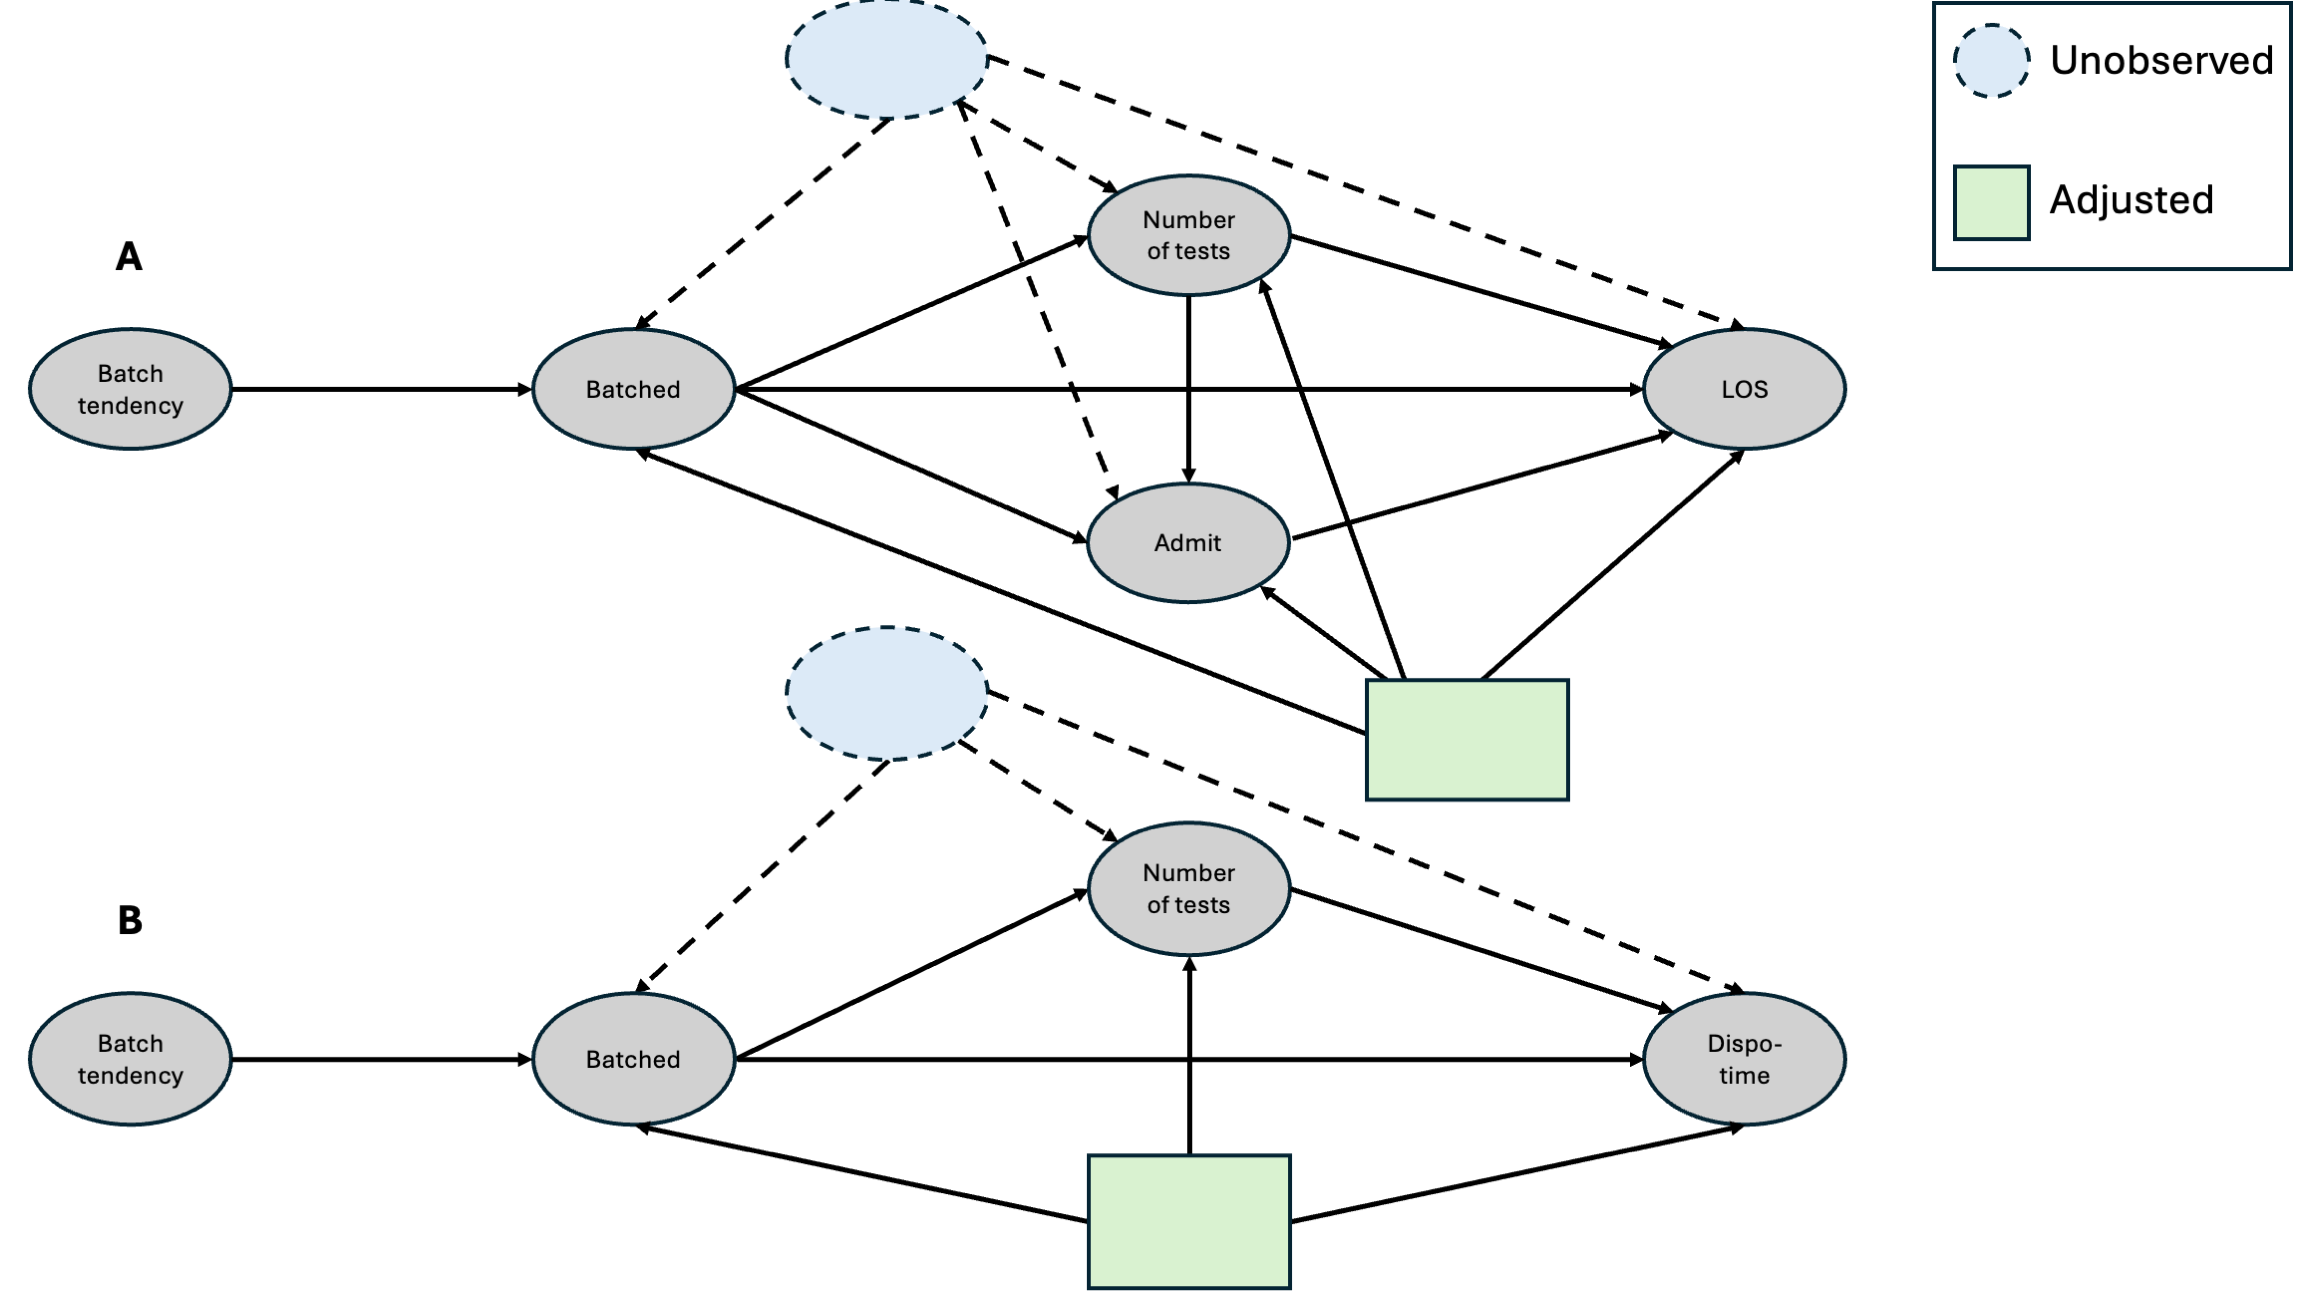
\includegraphics[width=\textwidth]{figures/dag.png}
\caption{Directed Acyclic Graph (DAG) of the Mediation Analysis}
\label{fig:dag}
\end{figure}

The mediation analysis results, detailed in Appendix Tables C1 and C2,
shed light on a plausible mechanism by which batching impacts LOS and
time to disposition. Our findings suggest that the effects of batching
are primarily mediated through increased diagnostic testing intensity.
This aligns with the results in Table \ref{tab:results_table},
demonstrating that batching increases imaging volume. This pathway
accounts for substantial delays in LOS, as additional imaging requires
time for completion, interpretation, and integration into clinical
decision-making. For LOS (Figure \ref{fig:dag} part A), the indirect
effect via imaging volume was estimated at \(0.207\) (\(p < 0.001\)),
indicating a substantial contribution to the total delay observed.
Similarly, for time to disposition (Figure \ref{fig:dag} part B), the
indirect effect via imaging was \(0.085\) (\(p < 0.001\)), underscoring
the central role of diagnostic testing intensity in extending processing
times. In contrast, the direct effects of batching on both LOS and time
to disposition were small and statistically insignificant, as shown in
Appendix Tables C1 and C2. This suggests that the delays attributed to
batching are driven not by the act of batching itself but rather by the
subsequent increase in diagnostic testing activity that batching
involves.

For LOS (Figure \ref{fig:dag} part A), the role of admission decisions
adds complexity to this narrative. Affirming the results in Table
\ref{tab:results_table}, the SEM analysis (Table C1) revealed that
batching was associated with a significant increase in admission
likelihood (\(b_2 = 0.327\), \(p < 0.001\)). This suggests that
increased imaging may contribute to more conservative disposition
decisions, potentially due to incidental findings or heightened
diagnostic uncertainty, which necessitate further inpatient care. This
pathway contributed to additional delays to LOS, as coordinating patient
transfers from the ED to inpatient units involves logistical challenges,
and further time consumption often accrued because of the lack of bed
availability in such units. The total indirect effect for LOS, combining
the pathways through imaging tests and admissions, was estimated at
\(0.256\) (\(p < 0.001\)), while the direct effect of batching remained
insignificant (\(c^\prime = 0.031\), \(p = 0.662\)). This consistency
between the 2SLS and SEM results (Table \ref{tab:results_table}, Table
C1, and Table C2 ) reinforces that diagnostic intensity and admission
are the key drivers of increased LOS in batched patients.

For time to disposition, where admission is not a mediator, the indirect
effect through imaging tests (\(0.085\), \(p < 0.001\)) remains the
predominant pathway, with the direct effect of batching again
nonsignificant (\(c^\prime = -0.100\), \(p = 0.216\)). This further
highlights that the perceived efficiency gains from batching outweigh
the operational burdens associated with increased diagnostic testing.

\subsection{Heterogeneous Effects: ED Capacity
Status}\label{heterogeneous-effects-ed-capacity-status}

Given that ED capacity constraints significantly influence operational
decisions, we examine whether batching's effects vary across different
capacity levels. Following The Mayo Clinic ED's internal
guidelines\footnote{The ED of our other partner hospital (MGH) does not follow these guidelines. Hence, we did not include these analyses in studying the effects of batching at MGH (see Section \ref{sec:generalize} for our analysis using MGH data).}
(Table A1), we categorize each encounter into three categories:
occurring during normal operations, minor overcapacity, or major
overcapacity. While our primary analysis controls for capacity status,
stratifying by this variable allows us to understand whether the impact
of batching on operational performance varies with ED congestion.

Table \ref{tab:het_effects} shows that batching's impact varies
significantly across ED congestion levels, with important implications
for operational efficiency. During normal operations, batching is most
frequent (15.8\% of encounters), leading to substantial increases in LOS
and time to disposition by 143\% and 125\%, respectively. Additionally,
batching is associated with an increase of 1.36 imaging tests per
patient. These findings suggest that when providers have greater
discretion, batching is used more liberally, contributing to
inefficiencies by increasing imaging volume and delaying result
turnaround.

As the ED enters minor overcapacity, batching frequency declines
slightly to 13.3\%, coinciding with the activation of workflow
interventions like the Rapid Medical Assessment (RMA) process (Table
A1). However, the adverse effects of batching remain pronounced, with
LOS increasing by 143\% and time to disposition by 144\%, while imaging
volume rises even further (+1.47 tests per patient). This suggests that
despite operational adaptations, providers continue using batching in a
way that exacerbates inefficiencies, likely because these interventions
do not directly constrain their ordering behavior.

A notable shift occurs under major overcapacity, where batching drops to
9.9\% of encounters, aligning with stricter constraints, such as
potential ED diversion and expedited bed assignments. Here, the adverse
effects of batching are markedly reduced, with nonsignificant LOS and
time to disposition increases. Imaging increases due to batching also
decline to 1.16 additional tests per patient. These results suggest that
providers use batching more selectively under extreme congestion, likely
reserving it for clinically necessary cases rather than as a
convenience.

These findings highlight how batching's impact depends on the ED's
operational state. When providers have more discretion, batching appears
most inefficient, driving up imaging volume and delays. Under severe
congestion, however, batching is less frequent and less detrimental,
suggesting a more strategic application. From a policy perspective,
interventions to curb batching should focus on normal and minor
overcapacity settings, where it contributes most to inefficiencies.

\begin{table}[t]
\centering
\caption{Heterogeneous Effects of Batching by ED Capacity Status}
\label{tab:het_effects}
\begin{threeparttable}
\begin{tabular}{lccc}
\toprule
& Normal & Minor & Major \\ 
& Operations & Overcapacity & Overcapacity \\ 
& (1) & (2) & (3) \\ 
\midrule
Log LOS & $0.890^{**}$ & $0.888^{*}$ & 0.534 \\ 
& (0.290) & (0.354) & (0.602) \\[0.5em] 
Log time to disposition & $0.812^{*}$ & $0.895^{*}$ & 0.742 \\ 
& (0.341) & (0.404) & (0.567) \\[0.5em] 
Number of distinct imaging tests & $1.355^{***}$ & $1.474^{**}$ & $1.160^{**}$ \\ 
& (0.088) & (0.398) & (0.357) \\[0.5em] 
72hr return with admission & -0.023 & -0.007 & 0.067 \\ 
& (0.012) & (0.032) & (0.067) \\[0.5em] 
\midrule
Batch mean & 0.158 & 0.133 & 0.099 \\[0.5em]
\\
Time FE & Yes & Yes & Yes \\ 
Baseline controls & Yes & Yes & Yes \\ 
Observations & 3,742 & 5,846 & 1,816 \\ 
\bottomrule
\end{tabular}
\begin{tablenotes}
\footnotesize
\item \textit{Notes:} This table reports two-stage least squares estimates of the impact of batching across different ED capacity levels. ED capacity levels are defined according to internal guidelines in Appendix Table A1. All specifications include time fixed effects and baseline controls. Robust standard errors clustered at the physician level are reported in parentheses. 
\item $^{*} p<0.05$, $^{**} p<0.01$, $^{***} p<0.001$.
\end{tablenotes}
\end{threeparttable}
\end{table}

\subsection{Determinants of Image
Batching}\label{determinants-of-image-batching}

To investigate the drivers of batching and image ordering behavior, we
examine the relationship between physician characteristics and ED
crowding and the likelihood of batched testing. We estimate the
following regression models:

\small

\begin{equation}
Y_{i,j} = \beta_0 + \mathbf{\beta_1 MD_j} + \gamma Capacity + \mathbf{\alpha X_{i}} + \epsilon_i
\end{equation}

\normalsize

Where \(Y_{i,j}\) represents our outcome of interest: Batched, a binary
measure of whether physician \(j\) batched tests for patient \(i\), and
the number of images ordered for patient \(i\) by physician \(j\).
\(\mathbf{MD_j}\) is a vector of physician characteristics, including
years since residency graduation, whether the physician is male, and the
number of hours they are into their shift. \emph{Capacity} is the
current capacity level of the ED, defined in Appendix Table A1.
\(\mathbf{X_{i}}\) is the vectors of patient covariates described in the
previous section and in Figure \ref{fig:batch_tendency}. We cluster
robust standard errors at the physician level. Table
\ref{tab:determinants} presents the results of the regression models.

\begin{table}[t]
\centering
\caption{\textbf{Determinants of Test Ordering Behavior}}
\label{tab:determinants}
\begin{threeparttable}
\begin{tabular}{p{8cm}cc}
\toprule
& Batched & Number of \\
& (1) & Imaging Tests (2) \\
\midrule
\multicolumn{3}{l}{\textit{Panel A. Physician Characteristics}} \\[0.5em]
Physician experience & -0.000 & -0.003 \\
& (0.002) & (0.002) \\[0.5em]
Physician male & 0.001 & 0.004 \\
& (0.029) & (0.041) \\[0.5em]
Hours into shift & $-0.004^{*}$ & -0.001 \\
& (0.002) & (0.003) \\[0.5em]
\multicolumn{3}{l}{\textit{Panel B. ED Conditions}} \\[0.5em]
Capacity Level: Minor overcapacity & -0.017 & -0.009 \\
& (0.010) & (0.013) \\[0.5em]
Capacity Level: Major overcapacity & $-0.047^{*}$ & -0.025 \\
& (0.017) & (0.024) \\[0.5em]
\midrule
Time FE & Yes & Yes \\
Baseline controls & Yes & Yes \\
Observations & 11,404 & 11,404 \\
$R^2$ & 0.044 & 0.093 \\
\bottomrule
\end{tabular}
\begin{tablenotes}
\footnotesize
\item \textit{Notes:} This table reports OLS estimates of the relationship between physician/ED characteristics and test ordering behavior. All specifications control for patient characteristics and time fixed effects. Robust standard errors clustered at the physician level are reported in parentheses. 
\item $^{*} p<0.05$, $^{**} p<0.01$, $^{***} p<0.001$.
\end{tablenotes}
\end{threeparttable}
\end{table}

We find that physician experience has no significant impact on batching
behavior, suggesting that more experienced physicians do not tend to be
more selective in their batching decisions. Additionally, physician
gender shows no significant relationship with batching or overall test
volume. However, the timing within a physician's shift significantly
influences batching decisions. Specifically, for each additional hour
into the physician's shift, the likelihood of batching tests decreases
by 0.3 percentage points (\(p<0.05\)). Because the Mayo Clinic ED
features very few handoffs, and physicians tend to stay with their
patients until disposition, this decline in batching as shifts progress
may reflect physicians adopting different testing strategies to ensure
they can complete their work before their shift ends.

ED capacity conditions also show interesting relationships with test
ordering patterns. Under major overcapacity conditions, we observe a
small but significant decreases in batching. This selective reduction in
testing during periods of high ED occupancy contrasts with previous
literature, suggesting that ED crowding prompts less discernment in the
use of diagnostic resources \citep{pines2009trends}.

\subsection{Generalizability of Results Across
EDs}\label{sec:generalize}

To assess the generalizability of our findings beyond the Mayo Clinic
ED, we replicated our analysis using data from the MGH ED, one of the
busiest emergency departments in the United States. The MGH dataset
comprises 129,489 patient encounters from November 10, 2021, through
December 10, 2022. This extensive dataset provides a robust sample to
validate the external applicability of our results.

Unlike the Mayo Clinic ED, where patients are randomly assigned to
physicians upon arrival through a rotational system, the MGH ED employs
a different patient assignment mechanism. At MGH, patients are triaged
into different care areas (e.g., urgent care, fast track, observation)
based on acuity and presenting complaints, then assigned to physicians
based on availability within those areas rather than through random
rotation. To address this non-random assignment and potential selection
bias, we adjust our instrumental variable strategy to account for these
differences by including additional covariates for care area assignment,
acuity level, and presenting complaints in both stages of our 2SLS and
instrument construction, thereby accounting for the sorting of patients
into different ED zones. While this approach cannot guarantee the same
level of causal identification as Mayo's randomized system, it provides
a more robust comparison of the effects of batching on patient outcomes
across different ED settings.

After adjusting for institutional differences and using the same
exclusion criteria we used with Mayo, we find strong evidence that our
key findings generalize to the MGH setting. The 2SLS results in Table
\ref{tab:generalize} suggest that batching leads to a 44.3\% increase in
length of stay and approximately 1.8 additional imaging tests per
patient. To formally assess whether the estimated effects differ
significantly across the two ED settings, we conduct a Z-test comparing
the 2SLS coefficients from MGH and Mayo by estimating:

\[
Z = \frac{\hat{\beta}{\text{MGH}} - \hat{\beta}{\text{Mayo}}}{\sqrt{SE_{\text{MGH}}^2 + SE_{\text{Mayo}}^2}}
\].

As reported in Column 4, the Z-statistics for each outcome indicate no
statistically significant differences in the estimated effects between
the two settings. This suggests that the impact of batching is mainly
consistent across hospitals despite differences in patient assignment
mechanisms and operational structures. Overall, these results reinforce
the external validity of our findings and provide further evidence that
the observed effects of batching are not merely an artifact of a single
institutions workflow but a systematic consequence of batching in
high-volume emergency care settings.

\begin{table}[t]
\centering
\caption{\textbf{Comparison of Effects of Batching Across Hospital Settings}}
\label{tab:generalize}
\begin{threeparttable}
\begin{tabular}{p{6cm}cccc}
\toprule
& \makecell{Sequenced \\ Mean (SD)} & OLS & 2SLS & \makecell{Z-Statistic} \\
& (1) & (2) & (3) & (4) \\
\midrule
Log LOS & 6.42 & $0.21^{***}$ & 0.34 & -0.907  \\
& (0.847) & (0.010) & (0.450) & \\[0.5em]

Number of distinct imaging tests & 1.34  & $0.780^{***}$ & $1.835^{***}$ & 1.23 \\
& (0.563) & (0.009) & (0.320) & \\[0.5em]

72hr return with admission & 0.0123  & $-0.0048^{***}$ & 0.0158 & 0.617  \\
& (0.110) & (0.001) & (0.038) & \\[0.5em]

\midrule
Time FE & --- & Yes & Yes & --- \\
Baseline controls & --- & Yes & Yes & --- \\
Observations & --- & 42,085 & 42,085 & --- \\
\bottomrule
\end{tabular}
\begin{tablenotes}
\footnotesize
\item \textit{Notes:} This table reports OLS and two-stage least squares estimates from the MGH dataset. All specifications include time fixed effects, baseline controls, and care area fixed effects. Robust standard errors clustered at the physician level are reported in parentheses. Column 1 reports the mean and standard deviation for non-batched patients (sequenced). Column 4 reports the Z-statistic from a formal test comparing the 2SLS coefficient in Column 3 to the 2SLS coefficient in Column 5 of Table \ref{tab:results_table}.
\item Significance levels: $^{***}p < 0.001$
\end{tablenotes}
\end{threeparttable}
\end{table}

\subsection{Managerial Implications}\label{managerial-implications}

Our findings have important implications for the management of ED
operations. First, while potentially appealing as a workflow efficiency
strategy, batch ordering of imaging tests can significantly increase ED
LOS and resource utilization without corresponding improvements in
patient outcomes. The substantial magnitude of these effects---an 130\%
increase in LOS for batched patients---suggests that ED managers should
carefully evaluate policies around physician test ordering discretion.
As our mediation analysis reveals, these delays arise primarily through
increased diagnostic intensity rather than the batching process itself,
indicating that sequential ordering may serve as a natural filter
against unnecessary testing.

The significant variation we observe in batching behavior across
physicians treating similar patients suggests an opportunity for
standardization. ED managers might consider implementing decision
support systems that encourage sequential ordering, particularly for
conditions where the information gained from initial tests frequently
eliminates the need for additional imaging. However, our heterogeneity
analysis indicates that such policies should be flexible to ED
conditions---the reduced impact of batching on test ordering during
periods of major overcapacity suggests that different strategies may be
optimal under varying capacity constraints. This would specifically be
the case if, for example, ED physicians consciously or subconsciously
avoid over-testing when they know resources are significantly limited.

The substantial cost implications of batch ordering---both in terms of
operational efficiency and resource utilization---suggest that EDs could
benefit from more structured approaches to test ordering. While
preserving physician autonomy in clinical decision-making is crucial,
our results indicate that completely unfettered discretion in test
ordering timing may lead to suboptimal system performance. Simple
interventions like providing feedback to physicians about their batching
rates relative to peers or implementing ``nudge'' systems that suggest
sequential ordering pathways could help reduce unnecessary testing while
maintaining the quality of care.

Finally, our findings have implications beyond individual EDs, as
increased admission rates from batch ordering create spillover effects
throughout the hospital system. Hospital administrators should consider
these downstream impacts when developing imaging protocols and resource
allocation strategies. Batching leads to increased testing and higher
admission rates, suggesting that policies aimed at reducing unnecessary
batch ordering could yield benefits across multiple dimensions of
hospital operations.

\subsection{Robustness Checks}\label{sec:robustness}

While our research design leverages the random assignment of patients to
physicians to identify causal effects, several limitations warrant
discussion. A primary concern is that physicians' tendency to batch
order tests may correlate with other unobserved practice patterns that
affect our outcomes of interest. Although we found no significant
associations between observable physician characteristics (such as
experience, gender, or training) and batch ordering tendency, unobserved
characteristics could influence both the tendency to batch and other
aspects of patient care. For instance, physicians who tend to batch
order tests might also have different approaches to patient assessment,
documentation practices, or consultation patterns that independently
affect the LOS and disposition decisions. Removing such unobserved
factors' potential impact might require running a fully randomized
experiment. However, the consistency and magnitude of our findings
across (a) both OLS and 2SLS specifications and (b) two different
hospitals with different practice settings provide strong evidence
behind our findings. In particular, unobserved physician characteristics
would need to be substantial to invalidate our core finding that
batching increases both test utilization and processing times.

Nevertheless, the validity of our results largely depends on our
identification strategy (Section \ref{sec:identification}). Thus, we
performed several robustness checks (see Appendix D) to gain further
confidence about the validity of our results. To provide robustness
checks related to potential exclusion restriction violations, we
adjusted for observable margins of care that may be correlated with the
tendency to batch, namely the decision to admit patients to the hospital
and the testing tendency of the physician (Appendix Table D2).
Additionally, we provide a placebo test where we check whether the
instrument has a positive first stage for a placebo outcome, namely the
number of laboratory tests ordered. Furthermore, we investigate whether
the reduced-form effects observed in Section \ref{sec:reducedform} are
due to differences in batch ordering rates across physicians or due to
other provider differences correlated with batch tendency. We examine
this by studying reduced-form effects among patients with conditions
that rarely require multiple imaging tests as a falsification check.
Finally, to address monotonicity, we follow approaches of
\citet{dobbie2018effects} and \citet{bhuller2020incarceration} and
construct physician-complaint-specific leniency instruments, and check
whether our instrument has a positive first stage across key complaint,
severity, capacity, and demographic-related subsamples (Appendix Figure
D1). Across all robustness checks and main outcomes, we found that the
magnitudes of our estimates remain fairly unchanged, and the
implications of our results remain consistent. Our robustness checks,
thus, give us further confidence about the validity of our main
findings. However, we acknowledge that a randomized experiment might
ultimately be needed to verify the results obtained from our
observational data.

\section{Conclusion}\label{conclusion}

Although prior literature examines task ordering from the perspective of
centralized protocols, frontline physicians often have discretion over
how and when they order diagnostic tests, especially in high-pressure
environments like EDs. In practice, due to system design or individual
choice, this delegation of decision-making results in physicians
self-managing their test-ordering strategies. Given the limited research
on the operational implications of test ordering, little is known about
how healthcare managers should guide these practices when such
discretion exists. Understanding when and how physicians exercise this
discretion informs decisions about system design, how to encourage
optimal use of discretion, and how to adjust policies to account for the
behaviors of frontline clinicians.

We explore this underexamined area by analyzing the drivers and
consequences of batch ordering imaging tests in the ED. Utilizing
detailed operational data from two large U.S. EDs, one with random
patient-physician assignment, we find that physicians are more likely to
batch order imaging tests earlier in their shifts and when the ED is
less crowded. This suggests that time pressure and occupancy levels
significantly influence the decision to batch, consistent with the
notion that physicians may adjust their ordering behavior based on their
workload and the operational demands of the ED.

Our results indicate that batch ordering imaging tests significantly
increase the number of imaging studies performed per patient encounter,
confirming that batching contributes to higher resource utilization.
However, we do not find evidence that batching reduces patient LOS in
the ED or impacts the likelihood of a 72-hour return with admission. On
the contrary, batching dramatically increases the time spent in the ED
and the time to disposition, suggesting that significant inefficiencies
from initiating multiple diagnostic imaging processes simultaneously
exist. This result aligns with previous research emphasizing the
importance of diagnostic pathways in achieving optimal health outcomes
and operational efficacy \citep[\citet{Masic2008},
\citet{Singh2015}]{Carpenter2015}. This is consistent with the
information gain advantage of sequential test ordering, where the
results of one test may eliminate the need for another. Our findings
suggest that discretion allows physicians to tailor their test ordering
to specific situations. However, it may also lead to resource-intensive
practices that do not benefit patients or the ED system.

Moreover, excess testing in EDs is not a benign phenomenon. It is
associated with increased risks, including patient exposure to
unnecessary radiation and the resultant psychological and physical
burden from incidental findings \citep{Mus2011}. Moreover, the economic
implications are substantial, with the overuse of diagnostic tests
contributing significantly to the escalating costs of healthcare
\citep{Atkinson2023}. As such, our results suggest the need to examine
the practice of batching across different clinical conditions and in
other clinical settings beyond the ED while also considering its
consequences across a variety of metrics that affect hospitals' publicly
reported outcomes \citep[\citet{saghafian2019role}]{Saghafian2019}.

Our study underscores the importance of developing evidence-based
guidelines to inform physicians' test ordering strategies. By
understanding how batching impacts patient outcomes and ED operations,
healthcare managers can design interventions to optimize test ordering
practices. This may include providing decision support tools, adjusting
policies to encourage sequential ordering when appropriate, or offering
feedback to physicians on their ordering patterns and associated
outcomes. By aligning physician test ordering strategies more closely
with patient needs \citep{Atkinson2023}, EDs may enhance patient
satisfaction and outcomes while improving operational efficiency.

\clearpage

% Appendix here
% Options are (1) APPENDIX (with or without general title) or
%             (2) APPENDICES (if it has more than one unrelated sections)
% Outcomment the appropriate case if necessary
%
% \begin{APPENDIX}{<Title of the Appendix>}
% \end{APPENDIX}
%
%   or
%
% \begin{APPENDICES}
% \section{<Title of Section A>}
% \section{<Title of Section B>}
% etc
% \end{APPENDICES}


% Acknowledgments here
\ACKNOWLEDGMENT{}

\bibliographystyle{informs2014}
\bibliography{references.bib}



\end{document}
